\section*{Introduction}
\phantomsection
   \addcontentsline{toc}{section}{Introduction}
   Ce rapport regroupe les points que j'ai préféré traiter au cours de l'UV MT94, vous y trouverez principalement des sujets en lien avec les deux parties sur les problèmes non-linéaires du cours. J'y décris les fondamentaux théoriques de chacune des notions abordées puis, je les applique sur Scilab avec des exemples plus concrets. Ce projet regroupe à la fois des notions introduites en TD, mais aussi des recherches personnelles plus approfondies sur certains points. \\\\
   Je tiens à remercier M.Stéphane Mottelet pour son accompagnement au cours du semestre et sa passion pour les mathématiques appliquées qu'il arrive à nous transmettre au travers de sa pédagogie.
      
      \markboth{Introduction}{}
    \newpage
 \section*{Problèmes non linéaires}
 \phantomsection
 \markboth{Problèmes non linéaires}{}
    \addcontentsline{toc}{section}{Problèmes non linéaires}
      Les problèmes mathématiques non linéaires sont tous les problèmes dont la sortie ne dépend pas linéairement de l'entrée. C'est à dire, les problèmes dont la sortie n'est pas proportionnelle à l'entrée ou ceux ne respectant pas le principe de superposition : 
      $\forall N \in \mathbb{N}$, soient $(f_i)_{i\in N}$ un ensemble d'entrées avec respectivement comme sortie $(x_i)_{i\in N}$ et $(\lambda_i)_{i\in N} \in \mathbb{R}^N$ un ensemble de nombres quelconques, alors la réponse à l'entrée $\sum_{i=1}^N \lambda_i f_i $ est : $ \sum_{i=1}^N \lambda_i x_i$. Ces problèmes peuvent être très long et coûteux à résoudre comme la recherche des zéros de polynôme de degré 4 ou supérieur. Il est donc dans ce cas plus simple d'approcher les solutions numériquement au détriment d'une précision absolue. La plupart des systèmes physiques étant non linéaires, la non linéarité est dense et possède de nombreuses applications. C'est pour cette raison que le cours de MT94 constitue deux chapitres sur la non-linéarité. Vous trouverez dans cette section plusieurs applications numériques sur ce sujet.
      \subsection{Les fractales}
         Commençons par nous intéresser au domaine passionnant que sont les fractales. Ces objets mathématiques complexes, à première vu désordonnés et aléatoires, sont en fait généralement générés à partir de simple équations et dont les conditions initiales peuvent faire complètement varier la figure obtenue. Leur particularité est leur structure caractérisée par des motifs similaires, les uns dans les autres, dont seule l'échelle varie.
         Cette caractéristique qui semble à priori uniquement visuelle et artistique, s'est aussi avéré intéressante dans de nombreux autres domaines d'application notamment en biologie pour la structure des plantes, en médecine pour celle d'organes comme les poumons ou encore en économie pour l'évaluation des risques financiers. Nous nous intéresserons dans cette section à quatre types de fractales générées par résolution de problèmes non linéaires.
         \subsubsection{La fractale de Newton}
            Pour construire la fractale de Newton, il faut utiliser la méthode de Newton. Pour rappel, cette méthode permet d'approximer le zéro d'une fonction $f$ en approximant localement sa tangente. En annulant la tangente on obtient ainsi facilement une première approche de la valeur cible. On calcul alors la nouvelle tangente de la fonction en ce point puis on réitère ce processus jusqu'à que l'on atteigne le rang k tel que $|f(x_k)|\leq tol$ avec $tol$ la précision définie initialement. 
            \\
            Soit un rang k, on suppose que $f$ est dérivable en $x_k$.
            Concrètement, si $f'(x_k) \neq 0$, on défini $x_{k+1}$ comme la solution de l'équation linéaire $$T(x) = 0,$$ avec $T(x) = f(x_k)+f'(x_k)(x-x_k)$, l'équation de la tangente de $f$ en $x_k$.
            \\
            \\
            On obtient donc
            $$x_{k+1} = x_k - \frac{f(x_k)}{f'(x_k)}.$$
            On peut coder la méthode de newton de cette manière sur Scilab : 

            \begin{center}
                \begin{minted}[breaklines, breakafter=-\{\}\%+-*]{scilab}
function x=newton(x0,tol,iteration_max)
    i=1;
    x=[];
    x(i)=x0;
    while abs(f(x(i)))>tol && i<iteration_max
        x(i+1)= x(i)-f(x(i))/fprime(x(i));
        //avec f et fprime la fonction et sa dérivée
        i=i+1;
    end
endfunction
                \end{minted}
               \captionof{listing}{Méthode de Newton}
               \label{lst:code_1}
            \end{center}

            Revenons en maintenant à la fractale de Newton. C'est un ensemble défini dans le plan complexe obtenu par l'application de la méthode de Newton dans le plan complexe à un polynôme $P(z), z\in \mathbb{C}$.
            \\ 
            On cherche donc à résoudre dans $\mathbb{C}$, l'équation
            $$P(z)=0.$$
            En utilisant la méthode de Newton, on définit la suite complexe récurrente $(z_n)$, 
            $$
            \forall n\in \mathbb{N}, (z_n) :
            \left\{
                \begin{array}{ll}
                    z_0\\
                    z_{n+1}=z_n-\frac{P(z_n)}{P'(z_n)}                    
                \end{array}
            \right..
            $$
        L'objectif est ainsi d'appliquer la méthode de Newton avec comme $z_0$, chacun des points d'une matrice obtenue à partir de la discrétisation d'un rectangle. Ainsi, avec un $z_0$ donné, la suite peut converger vers une des $d$ racines du polynôme avec d le degré de ce dernier ou ne pas converger du tout. Dans ce cas, on dit que $z_0$ appartient à la fractale de Newton. \\
        La fractale de Newton classique est celle obtenue pour le polynôme $P(z)=z^3-1$. Pour une première simulation sur Scilab, on va utiliser ce polynôme. Ainsi, notre suite $(z_n)$sera définie par
        $$
            \forall n\in \mathbb{N}, (z_n) :
            \left\{
                \begin{array}{ll}
                    z_0\\
                    z_{n+1}=z_n-\frac{z_n^3-1}{3z_n^2}                    
                \end{array}
            \right..
          $$
         On va définir, à partir de la discrétisation à $n^2$ points du rectangle $[-1, 1]\times [-1, 1]$, la matrice $Z=X+iY$ (le problème étant dans $\mathbb{C}$, il faut considérer partie imaginaire/réelle). Puis, pour chacun des points de Z, appliqués à la méthode de Newton, on définira une couleur parmi 3, en fonction de sa convergence, ou bien du blanc s'il ne converge pas vers une solution.
         \\
         \\
         Dans Scilab, l'application de la méthode de Newton pour ce problèmes se caractérisera par ce code :
         \begin{center}
                \begin{minted}[breaklines, breakafter=-\{\}\%+-*]{scilab}
tol = 1e-15;
n = 3e3;
[X,Y] = meshgrid(x,x);
Z = complex(X,Y);
for nombre_it=1:20
    Z=Z-((Z.^3)-1)/(3*Z.^2);
end
A = ones(n,n);
solutions = [1,-1/2+%i*(sqrt(3)/2),-1/2-%i*(sqrt(3)/2)];
//définitions des solutions exactes
for i = 1:3
    A(abs(Z-solutions(i))<tol) = i+1;
    //permet de déterminer si un nombre converge et de lui associer un nombre entre 2 et 4 si c'est le cas, ce qui sert pour la définition de la couleur
end
                \end{minted}
               \captionof{listing}{Adaptation de la méthode de Newton à la fractale de Newton }
               \label{lst:code_2}
            \end{center}
            Ici, on impose le nombre d'itération (20) afin de mettre en évidence les zones blanches de la fractale de Newton. La tolérance tol définie ici la limite que l'on fixe pour considérer qu'avec une condition initiale $z_0$ la suite converge vers une des racines. Ainsi, plus tol est élevée, moins les zones blanches seront grandes car un nombre plus élevé de valeurs seront considérées comme convergant vers une des solutions.
            \\
            A l'issue de ce programme on obtient la figure de fractale suivante :
            \begin{figure}[h]
              \centering
                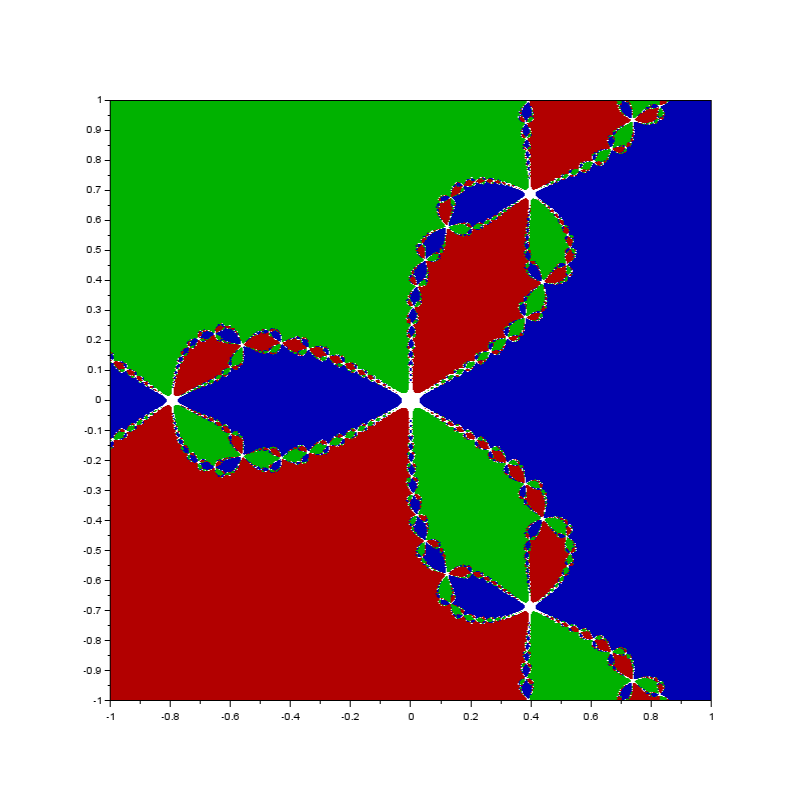
\includegraphics[width=0.8\textwidth]{images/fractale_newton1.png}
              \caption{Fractale de Newton pour $P(z) = z^3-1$ et $n=3000$}
              \label{fig:fractale_newton1}
            \end{figure}
            \\On peut ensuite généraliser notre programme à des polynômes de degrés $d$ quelconques ainsi qu'à une taille d'image de côté quelconque. Voici un programme Scilab complet et davantage généralisé :
            \begin{center}
                \begin{minted}[breaklines, breakafter=-\{\}\%+-*]{scilab}
function y = f(Z,d)
    y = (Z.^d)-1;
endfunction
function y = fprime(Z,d)
    y = d*(Z.^(d-1));
endfunction
tol = 1e-10;
n = 5e3;
d=3;
mini=-2;
maxi=2; // Valeurs entre lesquels seront constitués X et Y
[X,Y] = meshgrid(x,x);
Z = complex(X,Y);
for nombre_it=1:20
    Z=Z-(f(Z,d)./fprime(Z,d));
end
A = ones(n,n);
solutions = roots(%z^d-1);
// Permet d'approximer les racines d'un polynôme de manière relativement précise sur Scilab
for i = 1:length(solutions)
    A(abs(Z-solutions(i))<tol) = i+1;
end
clf;
basic_colors = [0.7 0 0; 0 0.7 0; 0 0 0.7; 0.7 0.7 0; 0 0.7 0.7; 0.7 0 0.7];
// Initialisation de la matrice de couleurs avec la première ligne blanche
colors = [1 1 1];
// Génération des couleurs aléatoires à partir de la graine 123 pour obtenir les mêmes couleurs à chaque fois
rand("seed", 123);
for i=1:d
    if i <= 6
        // Si d <= 6, on utilise les couleurs basiques dans l'ordre
        colors = [colors; basic_colors(i,:)];
    else
        // Sinon, on génère des couleurs aléatoires
        colors = [colors; rand(1, 3)];
    end
end
gcf().color_map = colors
plot(mini,mini,maxi,maxi)
Matplot1(A,[mini,mini,maxi,maxi])
isoview
                \end{minted}
               \captionof{listing}{Fractale de Newton de degré $d$}
               \label{lst:code_3}
            \end{center}
            Voici quelques exemple d'autres fractales de Newton obtenues avec ce programme ou avec de légères modifications : 
            \begin{figure}[h]
                \centering
                \begin{minipage}[b]{0.3\textwidth}
                    \includegraphics[width=\textwidth]{images/fractale_newton_degré5.png}
                    \caption{Fractale de Newton pour $P(z) = z^3-1$ et $n=3000$}
                    \label{fig:fractale_newton2}
                \end{minipage}
                \hfill
                \begin{minipage}[b]{0.3\textwidth}
                    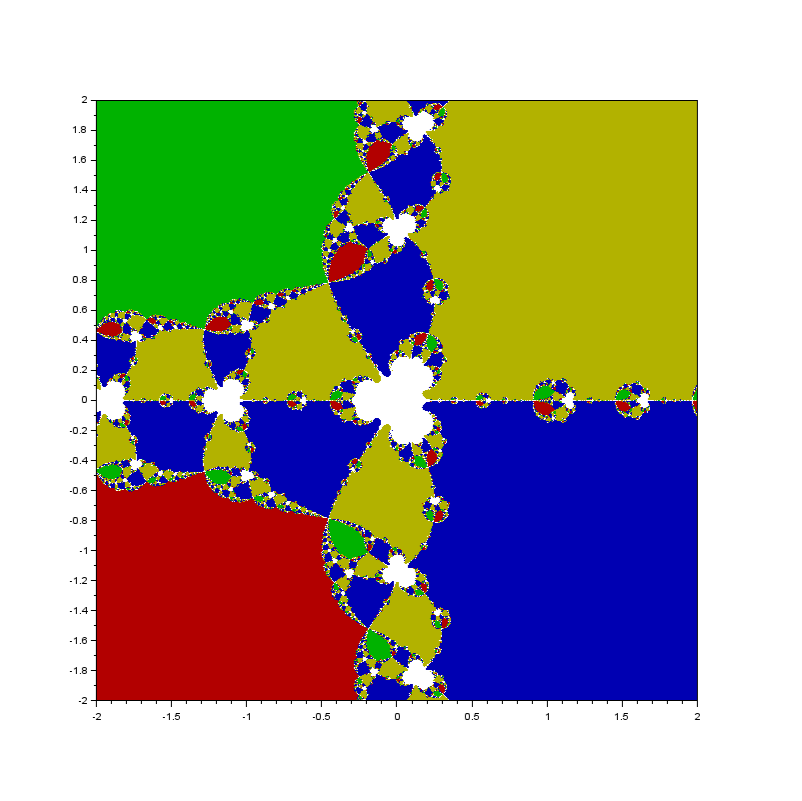
\includegraphics[width=\textwidth]{images/fractale_newton_z4-3z+5.png}
                    \caption{Fractale de Newton pour $P(z) = z^4-3z+5$ et $n=5000$}
                    \label{fig:fractale_newton3}
                \end{minipage}
                \hfill
                \begin{minipage}[b]{0.3\textwidth}
                    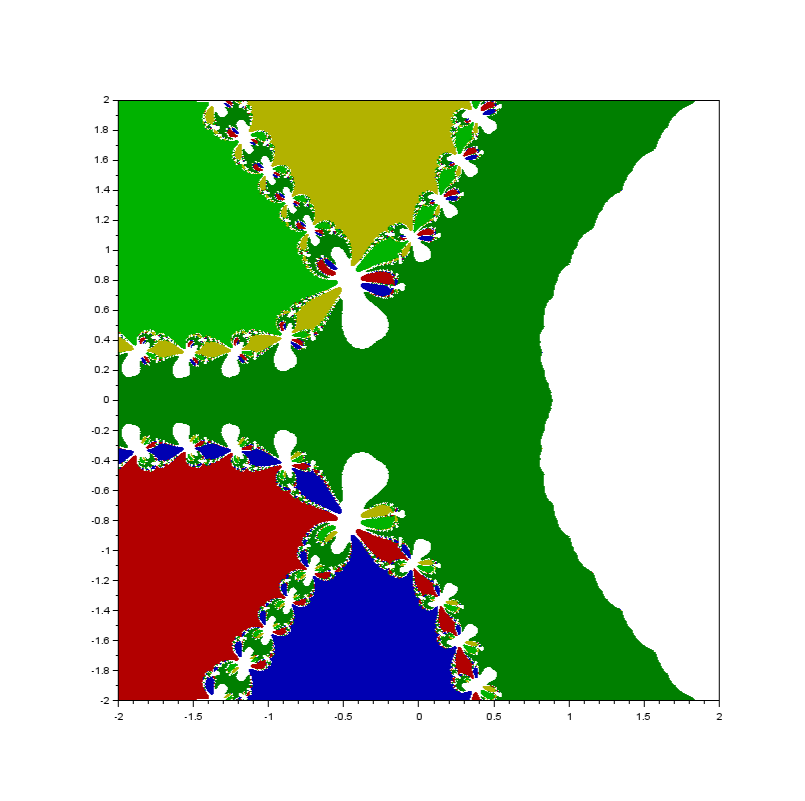
\includegraphics[width=\textwidth]{images/fractale_newton_z7-3z4+5z-3.png}
                    \caption{Fractale de Newton pour $P(z) = z^7-3z^4+5z-3$ et $n=3000$}
                    \label{fig:fractale_newton4}
                \end{minipage}
            \end{figure}

            
         \subsubsection{Ensemble de Mandelbrot}
         Intéressons nous maintenant à 2 autres modèles de fractale dont la génération est assez ressemblante : l'ensemble de Mandelbrot et de Julia.
         L'ensemble de Mandelbrot $\mathcal{M}$ est une fractale définie par l'ensemble des points $c$ du plan complexe tels que la suite $(z_n)_{n\geq 0}$ soit bornée.:
         $$(z_n)_{n\geq 0} :
            \left\{
                \begin{array}{ll}
                    z_0=0\\
                    z_{n+1}=z_n^2 + c                    
                \end{array}
            \right.
         $$
         Pour cela, on va montrer
         $$\exists n \geq 0, |z_n| > 2 \Rightarrow c \notin \mathcal{M}$$
        
         \begin{proposition}
            Soit $c \in \mathbb{C}$ tel que $|c| > 2$. Alors $|z_n(c)|\underset{n\to +\infty}{\longrightarrow}+\infty$, donc, $c\notin \mathcal{M}$.
         \end{proposition}
         \begin{preuve}
            On pose $|c| = 2+a$ avec $a>0$. On a $|z_0|=|c|=2+a$. \\Soit $n \in \mathbb{N}$. Supposons l'existence d'un réel $r_n > 0$ tel que $|z_n| \geq 2+r_n a$.
            \\Alors par inégalité triangulaire, 
            $$|z_{n+1}|=|z_n^2+c|\geq |z_n|^2-|c|\geq (2+r_n a)^2-(2+a)$$
            Or,
            $$(2+r_n a)^2 = 4 + 4 r_n a+r_n^2 a^2 \geq 4+4 r_n a$$
            Donc,
            $$|z_{n+1}| \geq  2+3 r_n a$$
            On en déduit pour tout $n>0$,
            $$|z_n|\geq 2+3^n a$$
            ainsi, $|z_n|$ tend vers $+\infty$ lorsque n tend vers l'infini.
         \end{preuve}
         \begin{proposition}
            Soit $c \in \mathbb{C}$ tel que $|c| \leq 2$. Supposons que pour un certain entier $n$ on ait $|z_n| > 2$. La suite $(z_n)_{n\geq 0}$ tend alors vers $+\infty$, et donc $c\notin \mathcal{M}$.
         \end{proposition}
         \begin{preuve}
            On pose $|z_n|=2+a$ avec $a>0$.\\On a par inégalité triangulaire,
            $$|z_{n+1}|=|z_n^2+c|\geq |z_n|^2-|c|\geq(2+a)^2-2\geq2+4a$$
            Par récurrence on montre ensuite, 
            $$\forall p \in \mathbb{N}|z_{n+p}|\geq 2+4^p a$$
            Ainsi $(z_n)_{n\geq 0}\underset{n\to +\infty}{\longrightarrow}+\infty$.
         \end{preuve}
         Ainsi, avec ces deux propositions on peut donc déduire que $$\exists n \geq 0, |z_n| > 2 \Rightarrow c \notin \mathcal{M}.$$ 
         Pour implémenter ceci dans Scilab et pouvoir ainsi dessiner l'ensemble de Mandelbrot, nous allons calculer par itération successive $z_n$ pour chacun des points $c$ issus de la discrétisation d'un rectangle (on choisira [-2,1] x [-1.5,1.5] en premier lieu pour observer la totalité de l'ensemble de Mandelbrot).\\ A chaque itération $k$, si le module de $z_k$ est supérieur à 2 pour une valeur de $c$, on lui attribue une couleur caractéristique. Les valeurs de $c$ pour lesquels le programme n'a pas détecté de divergence à partir d'un rang $n$ fixé resteront noir sur la figure finale.
         \\Le code suivant permet de générer l'ensemble de Mandelbrot en pouvant changer les coordonnées du centre du rectangle qui nous intéresse et sa valeur de zoom sur la fractale. A noter que j'ai créer un colormap personnalisé pour avoir un résultat plus esthétique mais qu'il en existe d'autres déjà fait que nous utiliseront par la suite.
         \begin{center}
                \begin{minted}[breaklines, breakafter=-\{\}\%+-*]{scilab}
function mandelbrot(x0, y0, zoom)
    n = 255; //nombre d'itérations du programme
    t = linspace(-1,1,2000) * 1.5 / zoom;
    t1 = t + x0;
    t2 = t + y0;
    [x, y] = meshgrid(t1, t2);
    c = x + %i * y;
    z = 0 * c;
    J = zeros(z); //matrice des couleurs initiallement noire
    for k = 1:n
        z = z.^2 + c;
        J((abs(z) > 2) & (J == 0)) = k; //on change la couleur de l'élément correspondant au c donné seulement si abs(z)>2 et si sa couleur n'a pas déjà été changée
        if modulo(k, 10) == 0 
            clf;
            Matplot(J); //on affiche toutes les 10 itérations pour voir l'évolution
            A = gca();A.isoview = "on";A.axes_visible = ["off" "off"];
        end
    end
    clf;
    Matplot(J);
    A = gca();A.isoview = "on";A.axes_visible = ["off" "off"];
endfunction
clf;F = gcf(); //définition du colormap personnalisé
colors = 256;
cmap = zeros(colors, 3);
for i = 1:colors
    ratio = (i-1) / (colors-1);
    if ratio <= 0.5
        cmap(i, :) = [ratio * 2, ratio * 2, 1];
    elseif ratio <= 0.85
        cmap(i, :) = [1, 1, 1 - (ratio - 0.5) * 2];
    else
        cmap(i, :) = [1, (1 - (ratio - 0.85) * 4), 0];
    end
end
F.color_map = cmap;
mandelbrot(-0.5,0,1) //Ensemble original
                \end{minted}
                \captionof{listing}{Ensemble de Mandelbrot}
                \label{lst:code_4}
         \end{center}
         \newpage
         A partir de ce programme on obtient cette figure :
         \begin{figure}[h]
              \centering
                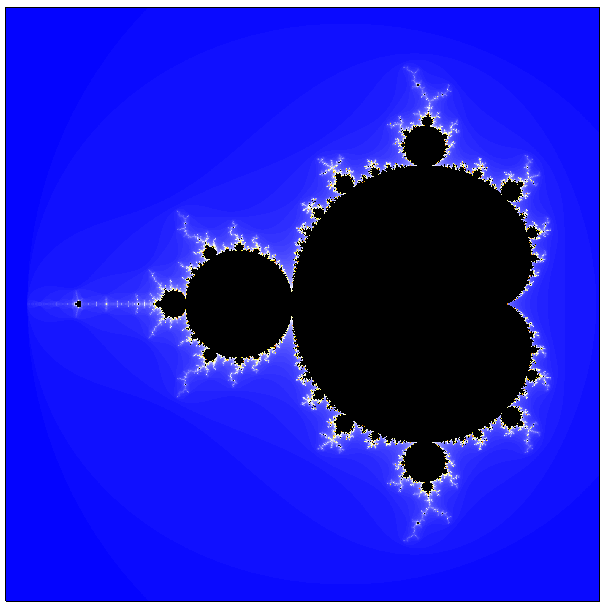
\includegraphics[width=0.6\textwidth]{images/Mandelbrot.png}
              \caption{Ensemble de Mandelbrot}
              \label{fig:mandel1}
            \end{figure}
        \\En jouant avec les valeurs de zoom et de coordonnées centrales ont peut aussi obtenir d'autres figures variées notamment en se rapprochant de la vallée des hippocampes :
         \begin{figure}[h]
                \centering
                \begin{minipage}[b]{0.3\textwidth}
                    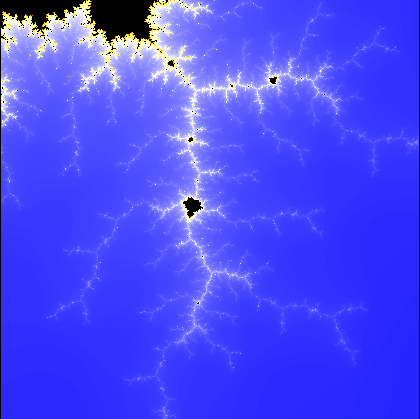
\includegraphics[width=\textwidth]{images/mandelbrot(-0.1528, 1.0397, 1000).png}
                    \caption{Centre en (-0.1528, 1.0397) avec un zoom de 1000}
                    \label{fig:mandel2}
                \end{minipage}
                \hfill
                \begin{minipage}[b]{0.3\textwidth}
                    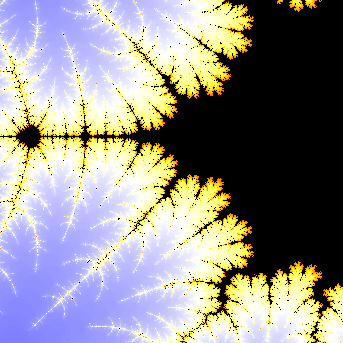
\includegraphics[width=\textwidth]{images/mandelbrot1(-1.401155, 0.000180, 2000).png}
                    \caption{Centre en (-1.401155, 0.000180) avec un zoom de 2000}
                    \label{fig:mandel3}
                \end{minipage}
                \hfill
                \begin{minipage}[b]{0.3\textwidth}
                    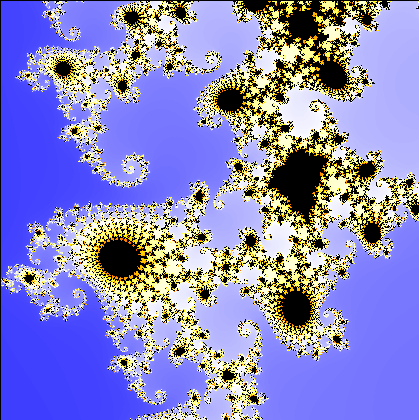
\includegraphics[width=\textwidth]{images/Mandelbrot1(-0.7463, 0.1102, 1000).png}
                    \caption{Centre en (-0.7463, 0.1102) avec un zoom de 1000}
                    \label{fig:mandel4}
                \end{minipage}
            \end{figure}
            \\
            On aurait pu également s'intéresser à d'autres polynôme que celui de la forme $z^2+c$ notamment en augmentant le degré ou en utilisant des fonctions trigonométriques.
            \newpage
         \subsubsection{Ensemble de Julia}
         La génération de l'ensemble de Julia est très similaire à celle  de Mandelbrot. En effet, pour une valeur $c$ fixée, l'ensemble de Julia correspond à la frontière de l'ensemble des valeurs initiales $z_0$ telles que la suite $(z_n)$ soit bornée :
         $$(z_n) : \left\{
                \begin{array}{ll}
                    z_0=0\\
                    z_{n+1}=z_n^2 + c                    
                \end{array}
            \right.$$
        \\ La principale différence à l'ensemble de Mandelbrot est donc le caractère fixe et unique de $c$.
         \\Voici un code Scilab permettant sa génération graphique (on utilise cette fois des colormap déjà implantés dans Scilab ce qui explique les variations de couleurs dans les figures suivantes :
         \begin{center}
                \begin{minted}[breaklines, breakafter=-\{\}\%+-*]{scilab}
function Julia(a,b,x0, y0, zoom)
    n = 85;
    t = linspace(-1,1,2000) * 1.2 / zoom;
    t1 = t + x0;
    t2 = t + y0;
    [x, y] = meshgrid(t1, t2);
    z = x + %i * y;
    c = a + %i*b; //valeur fixe
    J = zeros(z);
    for k = 1:n
        z = z.^2 + c;
        J((abs(z) > 2) & (J == 0)) = k;
    end
    clf;
    Matplot(J);
    A = gca();
    A.isoview = "on";
    A.axes_visible = ["off" "off"];
endfuction
                \end{minted}
                \captionof{listing}{Ensemble de Julia}
                \label{lst:code_5}
         \end{center}
            Les possibilités de représentations distinctes sont infinis avec ce programme. Voici quelques-unes des plus esthétiques  que j'ai pu obtenir :
            \begin{figure}[h]
                \centering
                \begin{minipage}[b]{0.45\textwidth}
                    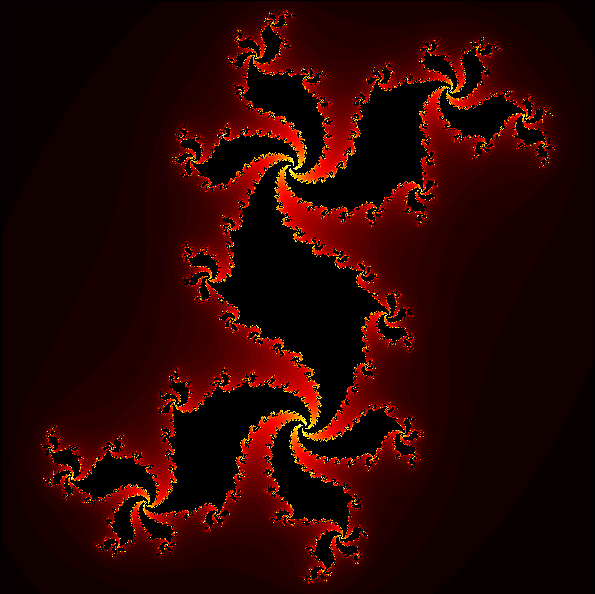
\includegraphics[width=\textwidth]{images/julia(c=(0.300000,0.500000xi)).png}
                    \caption{Ensemble de Julia pour c=0.3+0.5i (cmap: hot)}
                    \label{fig:julia1}
                \end{minipage}
                \hfill
                \begin{minipage}[b]{0.45\textwidth}
                    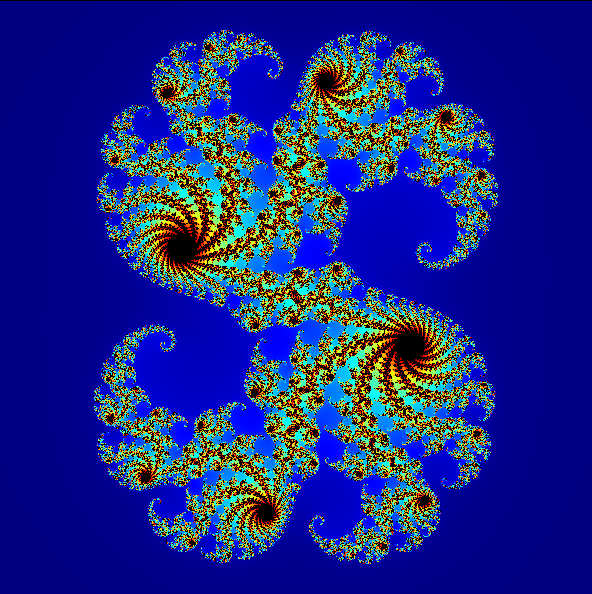
\includegraphics[width=\textwidth]{images/julia(c=(0.285000,0.013000xi)).png}
                    \caption{Ensemble de Julia pour c=0.285+0.013i (cmap: jet)}
                    \label{fig:julia2}
                \end{minipage}
            \end{figure}
            \begin{figure}[h]
                \centering
                \begin{minipage}[b]{0.45\textwidth}
                    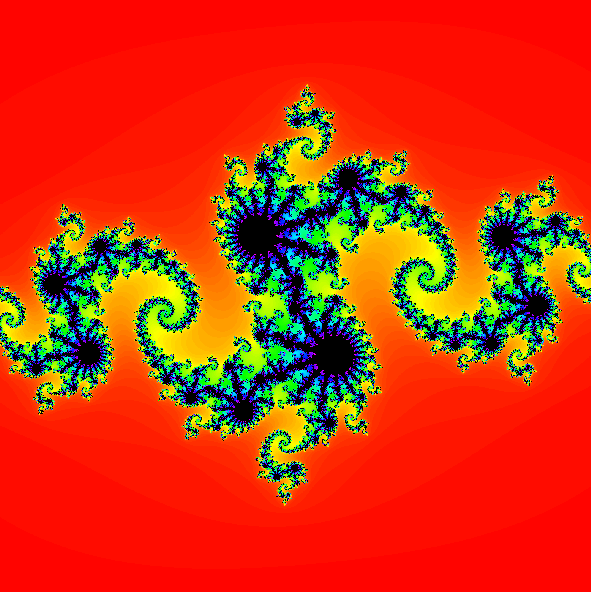
\includegraphics[width=\textwidth]{images/julia(c=(-0.800000,0.156000xi)).png}
                    \caption{Ensemble de Julia pour c=-0.8+0.156i (cmap: hsv)}
                    \label{fig:julia3}
                \end{minipage}
                \hfill
                \begin{minipage}[b]{0.45\textwidth}
                    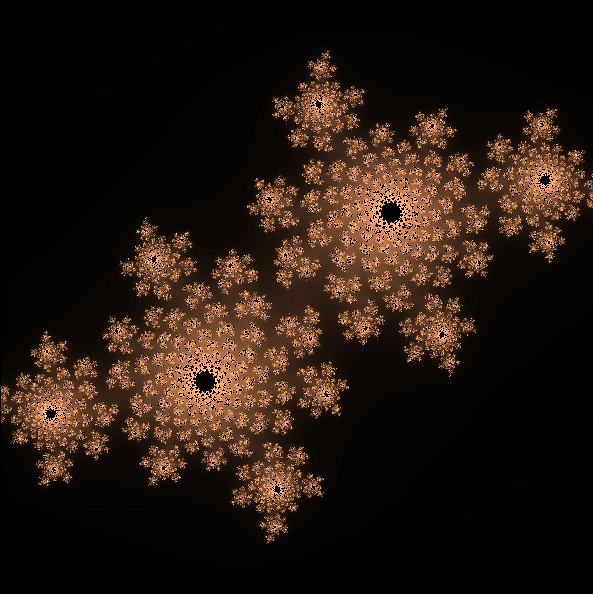
\includegraphics[width=\textwidth]{images/julia(c=(-0.400000,0.600000xi)).png}
                    \caption{Ensemble de Julia pour c=-0.4+0.6i (cmap: copper)}
                    \label{fig:julia4}
                \end{minipage}
            \end{figure}
            \newpage
      \subsection{Problèmes des moindres carrés linéaires}
      Les problèmes des moindres carrés linéaires sont des cas particulier des problèmes d'optimisation.
      \\Soit $S :\mathbb{R}^n \to \mathbb{R}$, on cherche $\hat{x}$ tel que : 
      $$S(\hat{x})\leq S(x), \forall x \in \mathbb{R}^n$$
         \subsubsection{Théorie}
         Pour utiliser la méthode des moindres carrés linéaires, il faut que le modèle $y = f_\theta (x)$ dépende linéairement des $\theta_j$ :
         $$f_\theta (x) = \sum_{j=1}^{p}\theta_j \phi_j(x), \phi_j : \mathbb{R} \to \mathbb{R}.$$
         L'objectif est ainsi de trouver les paramètres $\theta$ tels que le modèle "corresponde" le mieux au set de données que l'on souhaite approximer.
         \\
         Soit $(x_i,y_i)_{i=1,...,n}$ un jeu de données dans $\mathbb{R}$, la méthode des moindres carrés linéaires consiste donc à trouver $\hat{\theta}$ minimisant la somme des carrés des résidus (SCR), 
         $$S(\theta) = \sum^n_{i = 1}(y_i-f_\theta (x_i))^2$$
         c'est à dire tel que
         $$\forall \theta \in \mathbb{R}, S(\hat{\theta}) \leq S(\theta)$$
         On défini le vecteur résiduel $r(\theta)$, donné par $(r(\theta))_i = y_i - f_\theta(x_i)$, avec $S(\theta) = ||r(\theta)||^2.$
         \\\\
         \textbf{Exemple - régression linéaire simple :}
         \begin{figure}[h]
              \centering
              \captionsetup{font=small}
                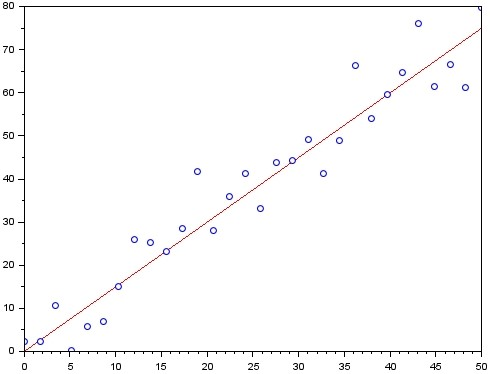
\includegraphics[width=0.4\textwidth]{images/regression_lineaire.jpg}
              \caption{Regression linéaire}
              \label{fig:reg1}
            \end{figure}
            \\
         Dans le cas d'une régression linéaire simple, on cherche donc $\theta_1, \theta_2 \in \mathbb{R}$ tels que la droite $y = \theta_1 x + \theta_2 = f_\theta(x)$ approche "au mieux" les données.\\ Soit la SCR associée, $$S(\theta) = \sum^n_{i=1}(y_i-(\theta_2 x + \theta_1)) = ||r(\theta)||^2$$
         Le vecteur résidu s'écrit alors
         $$r(\theta) = y - \theta_1 \begin{bmatrix}1 \\\vdots \\1 \\\end{bmatrix}
         - \theta_2\begin{bmatrix}x_1 \\\vdots \\x_n \\\end{bmatrix} = y - A\theta,$$
         Avec $y = \begin{bmatrix}y_1 \\\vdots \\y_n \\\end{bmatrix} $ et $A = \begin{bmatrix}1&x_1 \\\vdots&\vdots \\1&x_n \\\end{bmatrix}$.
         \\\\\\\textbf{Ainsi, de manière générale, on aura :} 
         $$
         r(\theta) = y - A\theta,
         $$
         $$
            y = \begin{bmatrix}y_1 \\\vdots \\y_n \\\end{bmatrix}, A = \begin{bmatrix}\phi_1(x_1)&\cdots&\phi_p(x_1) \\\vdots&\ddots&\vdots \\\phi_1(x_n)&\cdots&\phi_p(x_n) \\\end{bmatrix}
         $$
         \\On rappelle qu'on cherche $\hat{\theta}$ tel que $S(\theta)$ soit minimale. Une condition nécessaire est :
         $$\nabla S(\hat{\theta})=\Vec{0}.$$
         On calcul $\nabla S(\hat{\theta})$ en développant $S(\theta + h)$ :
         \begin{align*}
         S(\theta + h) &= ||y-A(\theta + h)||^2\\
         &=||(y-A\theta)-A h||^2\\
         &=||y-A\theta||^2-2(y-A\theta)^T A h+||A h||^2\\
         &=S(\theta)+S'(\theta)h+||A h||^2
         \end{align*}
         On a ainsi,
         $$S'(\theta) = -2(y-A\theta)^T A = \nabla S(\theta)^T.$$
         et donc,
         \begin{align*}
         \nabla S(\hat{\theta}) = \Vec{0} &\Leftrightarrow A^T(y-A\hat{\theta}) = \Vec{0}\\
         &\Leftrightarrow A^T A \hat{\theta} = A^T y
         \end{align*}
         \newpage
         Soit le théorème suivant :
         \begin{theoreme}
             Une solution du problème des moindres carrés est donnée par la résolution du système $A^T A\hat{\theta}=A^T y$, et si $rang(A) = p$, cette solution est unique.
         \end{theoreme}
        \begin{preuve}
        On écrit le développement de $S(\theta)$ en $\hat{\theta}$,
         \begin{align*}
             S(\theta) &= S(\hat{\theta}+(\theta - \hat{\theta}))\\
             &=S(\theta)+\nabla S(\hat{\theta})^T(\theta-\hat{\theta})+||A(\theta - \hat{\theta})||^2
         \end{align*}
         Avec $\nabla S(\hat{\theta}) = \Vec{0} $ et $ ||A(\theta - \hat{\theta})||^2\geq0$ \\d'où,
         $$\forall \theta \in \mathbb{R}, S(\theta) \geq S(\hat{\theta})$$
        Unicité : 
        \begin{align*}
            S(\theta) = S(\hat{\theta})&\Leftrightarrow A(\theta-\hat{\theta}) = \Vec{0}\\
            &\Leftrightarrow \theta = \hat{\theta}
        \end{align*}
        Avec $A$ de rang $p$
        \end{preuve}
        Sur Scilab, résoudre $A^T A\hat{\theta}=A^T y$  se traduira par l'expression $x=A\textbackslash y$ qui est équivalente mathématiquement à $x=(A'*A)\textbackslash (A'*y)$ mais plus stable, précise et efficace. On utilisera toujours $x=A\textbackslash y$ par la suite.
         \subsubsection{Régression polynomiale}
         Prenons ici un jeu de données, qu'on a pu générer à partir d'une fonction polynomiale à laquelle on a rajouté un bruit : 
         \begin{figure}[h]
              \centering
              \captionsetup{font=small}
                \includegraphics[width=0.51\textwidth]{images/données.jpg}
              \caption{Données issues d'un polynôme}
              \label{fig:reg2}
            \end{figure}
            \newpage
         Voici le code associé à cette représentation :
         \begin{center}
                \begin{minted}[breaklines, breakafter=-\{\}\%+-*]{scilab}
t=linspace(-4,3.25,400)';
y=(1/20)*t.^5+(3/20)*t.^4-(11/20)*t.^3-(27/20)*t.^2+(1/2)*t+(16/5);
rand("seed",1);
y=y+rand(400,1,'normal')./2;
plot(t,y,'o');
                \end{minted}
                \captionof{listing}{Génération bruitée d'un jeu de données relatif à un polynôme}
                \label{lst:code_6}
         \end{center}
         Pour approximer la fonction et résoudre le problème de moindres carrés, le programme va itérer sur le degré p afin de générer la matrice $A$ puis afficher le résultat, et ce, pour des valeurs croissantes de p. Voici le programme Scilab correspondant (il utilise les données créées précédemment (Code source 6): 
         \begin{center}
                \begin{minted}[escapeinside=||,mathescape=true,breaklines, breakafter=-\{\}\%+-*]{scilab}
A=[];
maxp=8;
for p=0:maxp
    for i=0:p
        A=[A, t.^i];
    end
    |$\theta$|=A\y;
    subplot(3, 3, p+1);
    plot(t,y,'o');
    plot(t, A*|$\theta$|,'r','thickness',2);
    title(sprintf("degré p=%d",p));
end
                \end{minted}
                \captionof{listing}{Génération des régressions pour différents degrés}
                \label{lst:code_7}
         \end{center}
         \newpage
         A partir de ce script on obtient ainsi pour les tracés pour les 8 premiers degrés : 
         \begin{figure}[h]
              \centering
                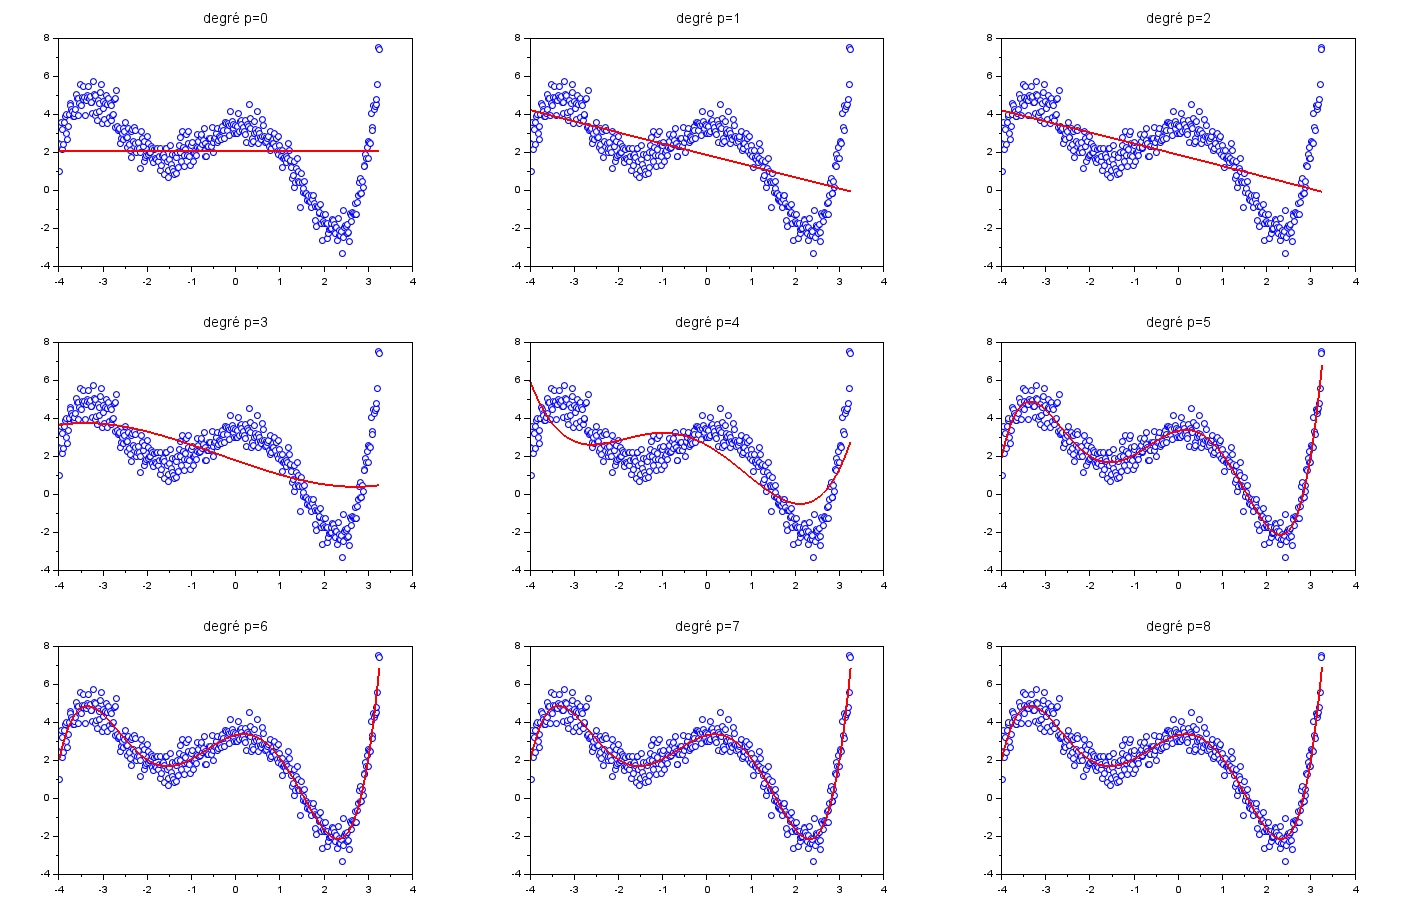
\includegraphics[width=1\textwidth]{images/reg.jpg}
              \caption{Régressions pour les 8 premiers degrés}
              \label{fig:reg3}
            \end{figure}
        \\
        A partir de ce résultat, on remarque que plus le degré augmente, plus l'approximation semble correcte. Cette observation est, en effet, correcte, et on verra que l'erreur résiduelle décroît en fonction du degré. Ainsi, on serait tenté de choisir le degré le plus élevé possible pour être sûr d'avoir une bonne approximation. Cependant, prendre un degré trop élevé n'est pas une solution adéquate car la régression ne serait alors plus efficace pour approximer de nouvelles données en dehors de l'espace d'entraînement de nos données actuelles. On peut donc se demander, comment choisir le degré optimal pour notre modèle ?
        \newpage
         \subsubsection{Choix du modèle}
          Pour trouver le bon degré, l'idée est alors de séparer les données en deux parties : un ensemble de travail et un ensemble de validation. L'ensemble de travail va être utiliser pour établir les modèles pour chacun des degrés que l'on souhaite essayer et l'ensemble de validation va faire office de nouvelles données qui n'ont pas servi pour l'entraînement du modèle pour ainsi comparer l'erreur résiduelle du modèle sur ces données et celle de l'ensemble de travail. On pourra alors sélectionner le degré pour lequel l'erreur est minime tant pour l'ensemble de travail que l'ensemble de validation.\\
          Soit le programme suivant en Scilab permettant de tracer la régression obtenue à partir de l'ensemble de travail (en bleu) sur l'ensemble des données et ainsi observer le potentiel écart du tracé avec l'ensemble de validation (en vert) : 
          {\fontsize{12}{11}\selectfont
          \begin{center}
          \captionsetup{font=small}
                \begin{minted}
                [escapeinside=||,mathescape=true,breaklines, breakafter=-\{\}\%+-*]{scilab}
clf
n = size(t)(1); //taille du vecteur t
T = floor(1/10*n:9/10*n); // on défini l'ensemble de travail (représente 8/10 du jeu de données)
V = setdiff(1:n,T); // complémentaire de T
errT=[];
errV=[];
A=[];
maxp=8;
for p=0:maxp
    for i=0:p
        A=[A, t.^i];
    end
    //on calcul theta seulement pour les lignes de A correspondant à l'ensemble de travail :
    |\theta|=A(T,:)\y(T);;
    //calcul de l'erreur résiduelle pour les 2 ensembles : 
    errT = [errT norm(A(T,:)*O-y(T))^2];
    errV = [errV norm(A(V,:)*O-y(V))^2];
    subplot(3, 3, p+1);
    plot(t,y,'o');
    plot(t(V),y(V),'go',t,A*O,'r','thickness',2);
    title(sprintf("degré p=%d",p));
end
clf;
plot('nl',0:maxp,errT,'-o',0:maxp,errV,'-o');
                \end{minted}
                \captionof{listing}{Génération des régressions avec validation pour différents degrés + calcul des erreurs}
                \label{lst:code_8}
         \end{center}
         }
         Voici les graphiques obtenus avec ce programme : 
         \begin{figure}[h]
              \centering
                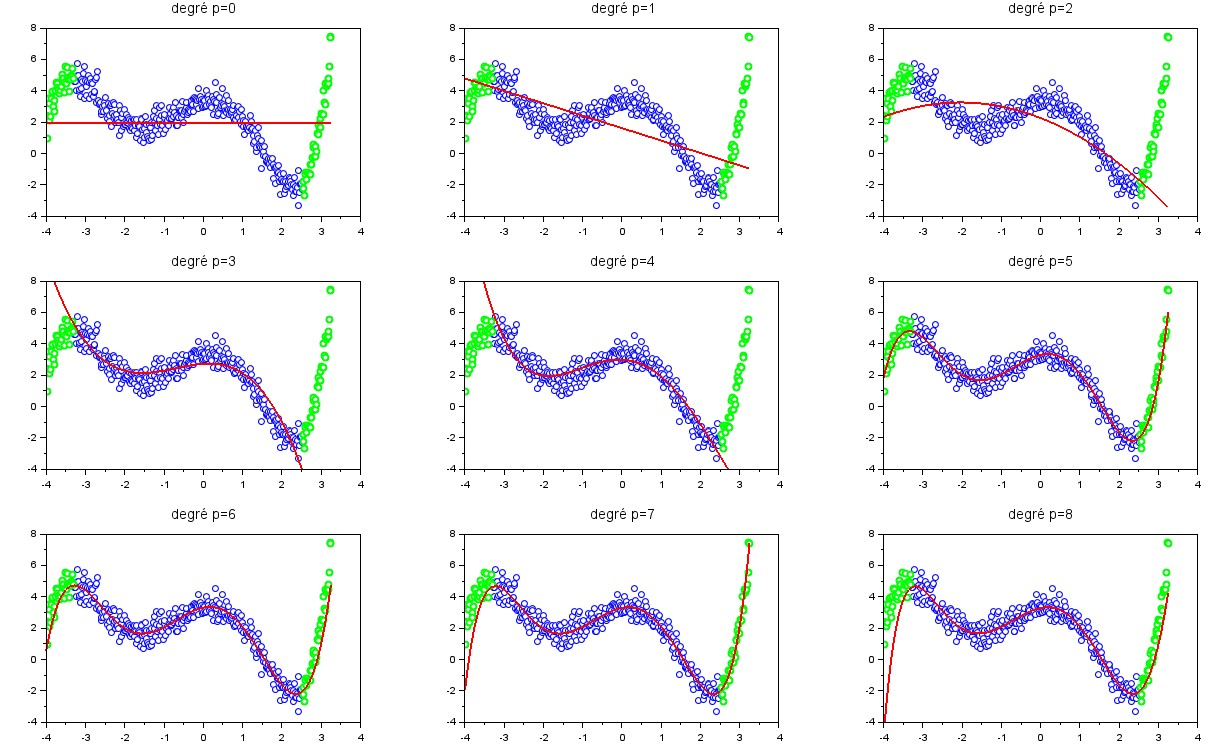
\includegraphics[width=1\textwidth]{images/reg_valid.jpg}
              \caption{Régressions et validations pour les 8 premiers degrés}
              \label{fig:reg4}
            \end{figure}
        \\
        Le choix de l'ensemble de validation est ici arbitraire (j'ai choisi le premier et le dernier dixième des t), cependant, un ensemble de travail trop court risque de donner lieu une régression peu précise et un ensemble de travail trop important par rapport à celui de validation atténuera la différence de précision entre les degrés.\\ Dans la figure ci dessus, on se rend bien compte qu'au degré 5, la courbe correspond à une bonne approximation puis que plus le degré augmente, plus l'erreur résiduelle avec l'ensemble de validation augmente.
        \\ On peut représenter cela en traçant le graphique du logarithme de l'erreur par rapport au degré afin d'identifier plus précisément le plus optimal : 
        \begin{figure}[h]
              \centering
              \captionsetup{font=small}
                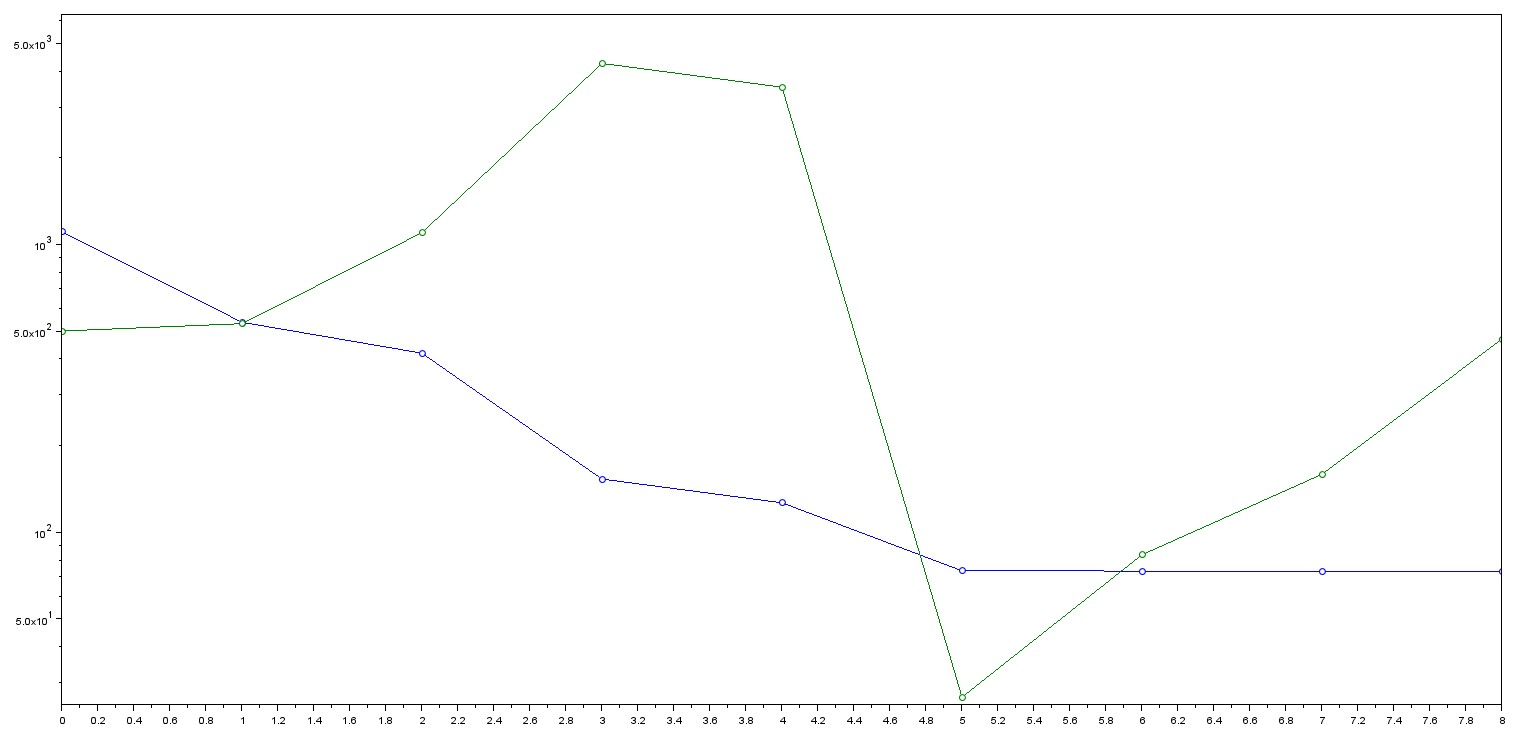
\includegraphics[width=0.8\textwidth]{images/erreur.jpg}
              \caption{Erreur résiduelle (validation et travail)}
              \label{fig:reg5}
            \end{figure}
        \\
        On observe ainsi, malgré la décroissance notable de l'erreur sur l'espace de travail, que l'erreur sur l'ensemble de validation ne suit pas la même évolution et atteint un minimum notable pour un degré égal à 5 qui est donc le degré optimal pour notre modèle. Au delà du degré 5, l'erreur de validation croît, on dit alors qu'il y a un surapprentissage car le modèle tend trop à correspondre aux données de l'ensemble de travail, se traduisant par une régression médiocre au delà. En effet, avec un degré égal au nombre de points dans notre set de données, il y aurait un passage par tous les points de la régression, ce qui ne nous intéresse pas ici.
        
         \subsubsection{Approximation d'un cercle}
         Outre les polynôme, il est également possible d'approximer des jeux de données par des objets mathématiques comme les cercles ou les ellipses, deux exemples que nous allons étudier maintenant.
         \\\\
         Pour trouver le cercle qui approxime le mieux les données $(x_i,y_i)_{i=1...n}$, l'objectif va être de minimiser la distance algébrique :
         $$d(a,b,R)=\sum_{i=1}^n ((x_i-a)+(y_i-b)-R^2)^2=||r||^2$$
         avec R le rayon du cercle et (a,b) les coordonnées du centre.\\\\ On rappelle qu'un cercle à pour équation $(x-a)^2+(y-b)^2=R^2$. Les paramètres ($a,b,R$) seront à trouver pour notre régression.\\
         \\Le vecteur résidu n'est pas linéaire par rapport à (a,b,r) mais on peut le développer ainsi pour une composante i quelconque : \\
         \begin{align*}
         r_i &= R^2 - a^2 -b^2 +2 a x_i + 2 b y_i - (x_i^2 + y_i^2)\\\\
         &=\begin{bmatrix}2x_i&2yi&1\end{bmatrix}\begin{bmatrix}a\\b\\R^2-a^2-b^2\end{bmatrix}-(x_i^2+y_i^2),
         \end{align*}
         De ce résultat, on peut donc affirmer que r est linéaire par rapport au vecteur $\theta=(a,b,R^2-a^2-b^2)$ qui est notre inconnu.
         On défini alors les matrices : 
         $$
         A=\begin{bmatrix}
             2x_1&2y_1&1\\
             \vdots&\vdots&\vdots\\
             2x_n&2y_n&1
         \end{bmatrix},
         z= \begin{bmatrix}
             x_1^2+y_1^2\\
             \vdots\\
             x_n^2+y_n^2
         \end{bmatrix},
         $$
         Telles que notre problème s'écrive :
         $$d(a,b,R)=||A\theta-z||^2.$$
         On peut alors définir $a=\theta(1),$ $ b=\theta(2) $ et $ R=\sqrt{\theta(3)+a^2+b^2}$. \\A partir de ces éléments, on peu ainsi construire le programme suivant en Scilab  :
         \begin{center}
          \begin{minted}[escapeinside=||,mathescape=true,breaklines, breakafter=-\{\}\%+-*]{scilab}
//génération du jeu de données
r = 3;
t = linspace(0,2*%pi,200)';
x = (r * cos(t));
y = (r * sin(t));
rand("seed",1);
y=y+rand(200,1,'normal')./4;
x=x+rand(200,1,'normal')./4;
clf;gca().data_bounds = [-4 -4 ;4 4];isoview on ;
//régression :
A=[2*x,2*y,ones(x)];
z=x.^2+y.^2;
|\theta|=A\z;
a=|\theta|(1);b=|\theta|(2);
R=sqrt(|\theta|(3)+a^2+b^2);
t=linspace(0,2*%pi,100);
plot(x,y,"o");
plot(a+R*cos(t),b+R*sin(t),'r','thickness',2);
          \end{minted}
                \captionof{listing}{Génération d'une régressions pour approximer des données par un cercle}
                \label{lst:code_9}
         \end{center}
         \newpage
        Le résultat obtenu est : 
        \begin{figure}[h]
              \centering
              \captionsetup{font=small}
                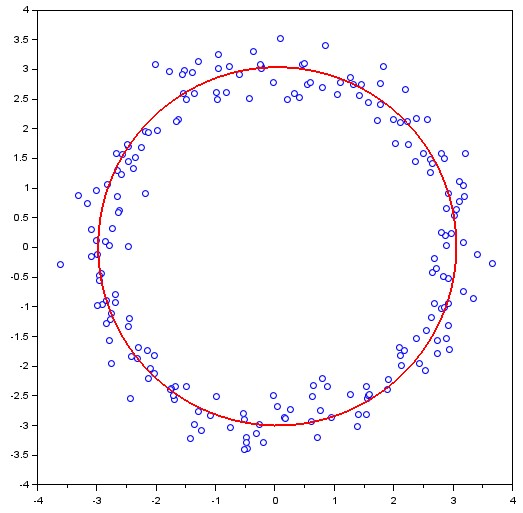
\includegraphics[width=0.5\textwidth]{images/cercle.jpg}
              \caption{Régression utilisant un cercle}
              \label{fig:reg6}
            \end{figure}
         \subsubsection{Approximation d'une ellipse}
         De la même manière que pour un cercle, pour approximer des données expérimentales $t_i = (x_i,y_i), i\in \llbracket 1,n\rrbracket$, par une ellipse, il faut minimiser la distance algébrique
         $$d(\alpha,\beta,\gamma,c_1,c_2)=\sum_{i=1}^n ((t_i-c)^T M(t_i-c)-\gamma^2)^2=||r||^2$$
         avec $c=(c_1,c_2)^T$ les coordonnées du centre de l'ellipse,$r$ le vecteur résidu et $ M=\begin{pmatrix}1&\alpha\\\alpha&\beta\end{pmatrix} $ la matrice définie positive. M à ses valeurs propres positives donc son déterminant l'est également ainsi que sa trace. Comme $det(M) = \beta - \alpha^2>0$ on a alors $\beta>\alpha^2.$\\
         De la même manière que pour le cercle, le vecteur résidu n'est pas linéaire par rapport à $(\alpha, \beta, \gamma, c_1,c_2)$, la difficulté est donc ici dans le nombre de paramètres inconnus à trouver qui est supérieur à celui du cercle.
         \\Développons et factorisons une composante i de r :
         \begin{align*}
             r_i&=t_i^TMt_i-2t_i^TMc+c^TMc-\gamma^2\\
             &=x_i^2+2\alpha x_iy_i+\beta y_i^2-2x_i(c_1+\alpha c_2)-2y_i(\alpha c_1+\beta c_2)+c^TMc-\gamma^2\\
             &=x_i^2 + (2x_iy_i,y_i^2,-2x_i,-2y_i,1)(\alpha,\beta,c_1+\alpha c_2, \alpha c_1+\beta c_2,c^TMc-\gamma^2)^T
         \end{align*}
         On peut ainsi écrire $r = Ap-b$ avec $b=\begin{bmatrix}-x_1^2\\\vdots\\-x_n^2         
         \end{bmatrix}, A = \begin{bmatrix}
             2x_1y_1&y_1^2&-2x_1&-2y_1&1\\
             \vdots&\vdots&\vdots&\vdots&\vdots\\
             2x_ny_n&y_n^2&-2x_n&-2y_n&1
         \end{bmatrix}$ \\\\et $p=(\alpha,\beta,c_1+\alpha c_2, \alpha c_1+\beta c_2,c^TMc-\gamma^2)^T$.
         \\Par définition, on a bien $\alpha = p_1$ et $\beta = p_2$. Ensuite, $p_5$ nous permet de calculer $\gamma$ : $\gamma^2 = c^TMc-p_5$. Enfin, on peut déduire de $p_3$ et $p_4$ le systèmes équations suivantes :
         \begin{align*}
         &p_3 = c_1 + \alpha c_2,\\
         &p_4 = \alpha c_1 + \beta c_2.
         \end{align*}
         ie : 
         $$
         Mc=\begin{pmatrix}
             p_3\\p_4
         \end{pmatrix}
         $$
         Il suffira ensuite de résoudre cette équation avec l'opérateur $[\textbackslash]$ dans Scilab.\\
         Pour tracer l'ellipse qui nous intéresse pour notre problème, on passe dans la base des vecteurs propres de la matrice $M$. Il existe donc une matrice orthogonale $P$ telle que la diagonalisation de $M$ s'écrive $D=P^TMP$ avec 
         $$
         D = \begin{pmatrix}
             \lambda_1&0\\
             0&\lambda_2
         \end{pmatrix}
         $$\\
         A partir de cela, il faut placer l'ellipse dans le bon repère, c'est à dire la centrer et utiliser les axes correspondant au repère propre. On pose donc le changement de repère suivant : $t=c+Pu$ avec u les nouvelles coordonnées. L'équation implicite de l'ellipse s'écrit alors : 
         \begin{align*}
             (t-c)^TM(t-c)&=u^TP^TMPu\\
             &=u^TDu\\
             &=\lambda_1u_1^2+\lambda_2u_2^2\\
             &=\gamma^2.
         \end{align*}
         On en déduit le paramétrage $u=\begin{pmatrix}
             \frac{\gamma}{\sqrt{\lambda_1}} \cos{k}\\
              \frac{\gamma}{\sqrt{\lambda_2}} \sin{k}
         \end{pmatrix}$, et ainsi dans le repère initial on a :\newpage
         $$
          t = c + \gamma P\begin{pmatrix}
              \frac{\cos{k}}{\sqrt{\lambda_1}}\\
              \frac{\sin{k}}{\sqrt{\lambda_2}}
          \end{pmatrix}
         $$
         A partir de tous ces éléments, on peut réaliser un programme Scilab permettant d'approximer un jeu de données par une ellipse (on utilisera un set de données construit de la même manière que dans les codes source 6 et 9 mais adapté à un ellipse) :
         \begin{center}
          \begin{minted}[escapeinside=||,mathescape=true,breaklines, breakafter=-\{\}\%+-*]{scilab}
A = [2*x.*y, y.^2,-2*x,-2*y,ones(x)];
p = A\(-x.^2);
a = p(1);
b = p(2);
M = [1 a; a b];
C = M\p(3:4);
|\gamma| = sqrt(C'*M*C-p(5));
[P,D] = spec(M); \\spec permet de calculer les vecteurs et valeurs propres d'une matrice
k = linspace(0,2*%pi,500);
\\calcul de Pu :
X = |\gamma|*P*[cos(k)/sqrt(D(1,1)); sin(k)/sqrt(D(2,2))] 
plot(x,y,'o');
plot(C(1)+X(1,:),C(2)+X(2,:), 'r',"thickness",3);
          \end{minted}
                \captionof{listing}{Génération d'une régressions pour approximer des données par une ellipse}
                \label{lst:code_10}
         \end{center}
         \newpage
         Ce qui nous permet d'obtenir par exemple la régression suivante :
         \begin{figure}[h]
              \centering
                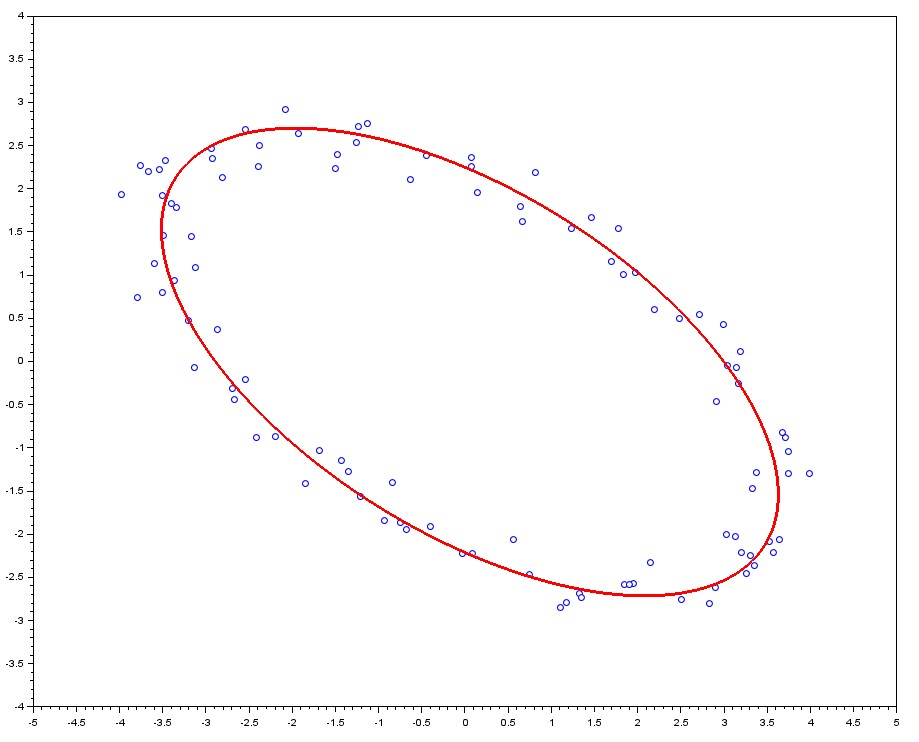
\includegraphics[width=0.8\textwidth]{images/ellipse.jpg}
              \caption{Régression utilisant une ellipse}
              \label{fig:reg7}
            \end{figure}
      \subsection{Problèmes des moindres carrés non linéaires}
      Après avoir vu comment résoudre des problèmes de moindres carrés linéaires, nous allons désormais généraliser cela pour des problèmes de moindres carrés non linéaires.
      \subsubsection{Première approche}
      On considère un jeu de donnés $(x_i,y_i)$ à approximer avec le modèle non linéaire 
      $$y=f_{\theta}(x)=exp(\theta_1 + \theta_2x),$$
      Similairement aux problèmes de moindres carrés linéaires, l'objectif va être de trouver un minimum local de $S(\theta) = ||r(\theta)||^2$.\\
      L'idée va être, dans le même esprit que la méthode de Newton, de trouver l'approximation affine du résidu de $S(\theta)$. On va donc considérer le développement de Taylor de ce résidu pour un vecteur qu'on appellera $\theta_k$
      $$r(\theta) = r(\theta_k)+r'(\theta_k)(\theta-\theta_k)+||\theta-\theta_k||\epsilon(\theta-\theta_k)$$
      On se place en fait dans un cadre itératif. L'objectif va être de déterminer le vecteur $\theta_{k+1}$ permettant de minimiser la norme au carré de son approximation affine :
      $$||r(\theta_k)+r'(\theta_k)(\theta_{k+1}-\theta_k)||^2$$
      Or, résoudre cette nouvelle formule revient simplement à résoudre un problème des moindres carré linéaire.\\
      \\Cette expression est en fait une formulation de la méthode de Gauss-Newton qui s'écrit 
      $$\theta{k+1}=\theta_k-[r'(\theta_k)^Tr(\theta_k)]^{-1}r'(\theta_k)^Tr(\theta_k),$$
      Avec comme simple équivalent Scilab :
      \begin{center}
          \begin{minted}[escapeinside=||,mathescape=true,breaklines, breakafter=-\{\}\%+-*]{scilab}
|\theta_{k+1}|=|\theta_k|-rprime(|\theta_k|)\r(|\theta_k|)
          \end{minted}
                \label{lst:code_11}
         \end{center}
         Le problème avec cette méthode est que pour avoir une solution unique, il est nécessaire que la matrice $r'(\theta_k)$ soit de rang maximal.
      \subsubsection{La méthode de Levenberg-Marquardt}
      \label{subsubsec:LM}
      Pour remédier au problème précédent apparu avec la méthode de Gauss-Newton, on utilise la méthode de Levenberg-Marquardt qui consiste à rajouter un terme supplémentaire à la fonction que l'on cherche à minimiser à chaque itération. On choisit un $\lambda > 0$ tel que 
      $$S_\lambda(\theta_k-\theta_{k+1}) = ||r(\theta_k)+r'(\theta_k)(\theta_{k+1}-\theta{k})||^2+\lambda||(\theta_{k+1}-\theta_k)||^2$$
      On peut réécrire cette expression en raisonnant par bloc
      $$S_\lambda(\theta_k-\theta_{k+1}) = \left\lVert \begin{pmatrix}
          r'(\theta_k)\\
          \lambda^{\frac{1}{2}}I
      \end{pmatrix}(\theta_{k+1}-\theta_k)+\begin{pmatrix}
          r(\theta_k)\\0
      \end{pmatrix}\right\rVert^2$$
      Ce problème reste donc linéaire mais possède toujours une unique solution quelque soit $\lambda>0$ contrairement à la méthode de Gauss-Newton.
      \\\\
      Le vecteur résidu s'écrit : 
      $$\begin{pmatrix}
          r'(\theta_k)\\
          \lambda^{\frac{1}{2}}I
      \end{pmatrix}(\theta_{k+1}-\theta_k)+\begin{pmatrix}
          r(\theta_k)\\0
      \end{pmatrix}$$
      On développe l'expression des équations normales : 
      $$
      \begin{pmatrix}
         r'(\theta_k)\\
         \lambda^{\frac{1}{2}}I
      \end{pmatrix}^T
      \begin{pmatrix}
          r'(\theta_k)\\
          \lambda^{\frac{1}{2}}I
      \end{pmatrix}(\theta_{k+1}-\theta_k)=-\begin{pmatrix}
         r'(\theta_k)\\
         \lambda^{\frac{1}{2}}I
      \end{pmatrix}^T
      \begin{pmatrix}
          r(\theta_k)\\0
      \end{pmatrix}
      $$$$\Leftrightarrow
      (r'(\theta_k)^Tr'(\theta_k)+\lambda I)(\theta_{k+1}-\theta_k)=-r'(\theta_k)^Tr(\theta_k)
      $$
      On formule ainsi les itérations de la méthode de Levenberg-Marquardt
      $$
      \theta_{k+1} = \theta_k - [r'(\theta_k)^Tr'(\theta_k)+\lambda I]^{-1}r'(\theta_k)^Tr(\theta_k)
      $$
      Sur Scilab, cette expression sera implémentée en utilisant l'opérateur $[\textbackslash]$ selon l'expression suivante : 
      $$
      \theta_{k+1} = \theta{k} - \begin{pmatrix}
          r'(\theta_k)\\ \lambda^{\frac{1}{2}}I
      \end{pmatrix}\textbackslash \begin{pmatrix}
          r(\theta_k)\\0
      \end{pmatrix}.
      $$
      Pour appliquer cette méthode à un problème concret, considérons la fonction de Rosenbrock, définie par
      $$f(x)=(1-x_1)^2+100(x_2-x_1^2)^2$$
      Pour mieux représenter le problème, il faut commencer par tracer les courbes iso-valeurs de $f$, c'est à dire la famille de courbes 
      $$C_\alpha = {x\in \mathbb{R}^2, f(x) = \alpha},$$
      avec $\alpha \geq 0$.
      On résout simplement le système : 
      \begin{align*}
          f(x) = \alpha &\Leftrightarrow (1-x_1)^2+100(x_2-x_1^2)^2=\alpha\\
          &\Leftrightarrow(\frac{1-x_1}{\sqrt{\alpha}})^2+(10\frac{x_2-x_1^2}{\sqrt{\alpha}})^2=1,
      \end{align*}
      On pose $$
      \frac{1-x_1}{\sqrt{\alpha}} = \cos{t}, 10\frac{x_2-x_1^2}{\sqrt{\alpha}}=\sin{t}, \forall t \in [0,2\pi],
      $$
      On obtient ainsi le paramétrage de $C_\alpha$ pour $t\in [0,2\pi]$: 
      $$
      x_1(t) = 1 - \sqrt{\alpha}\cos{t},
      $$
      $$
      x_2(t) = \frac{\sqrt{\alpha}}{10}\sin{t}+x_1(t)^2,
      $$
      En Scilab, le tracé de ces courbes se traduit par le code suivant : 
      \begin{center}
          \begin{minted}[escapeinside=||,mathescape=true,breaklines, breakafter=-\{\}\%+-*]{scilab}
clf;
isoview ;
gca().data_bounds=[-1.5 2.5 -1.5 2.5]; //permet d'observer les courbes uniquement dans le domaine [-1.5,2.5]x[-1.5,2.5]
gca().auto_scale='off'; //nécessaire pour empêcher la figure de modifier sa taille par la suite
t=linspace(0,2*%pi,1000);
for alpha=1:10:500 //on défini le nombre de courbes à afficher et l'espacement
    x1 = 1-sqrt(alpha)*cos(t);
    x2 = sqrt(alpha)/10*sin(t)+x1.^2;
    plot(x1,x2);
end
          \end{minted}
                \captionof{listing}{Tracé des courbes iso-valeurs de la fonction de Rosenbrock}
                \label{lst:code_12}
         \end{center}
         A partir de ce code on obtient ainsi la figure suivante : 
         \begin{figure}[h]
              \centering
              \captionsetup{font=small}
                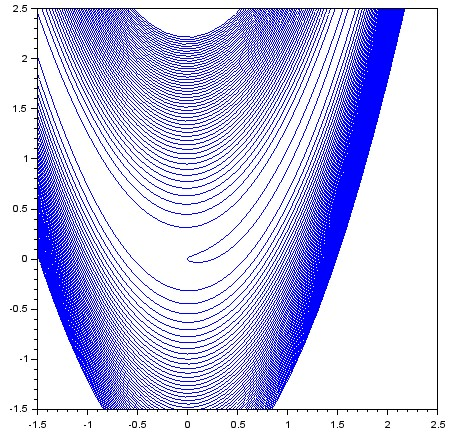
\includegraphics[width=0.6\textwidth]{images/rosenbrock.jpg}
              \caption{Courbes iso-valeurs de la fonction de Rosenbrock}
              \label{fig:LM1}
            \end{figure}
            \\
        Pour appliquer la méthode de Levenberg-Marquardt, on doit calculer les résidus et la matrice jacobienne associée. On a $$
        f(x)=(1-x_1)^2+(10(x_2-x_1^2))^2 = ||r(x)||^2
        $$
        Donc le vecteur résidu s'écrit 
        $$
        r(x) = \begin{pmatrix}
            1-x_1\\10(x_2-x_1^2)
        \end{pmatrix}
        $$
        et
        $$
        r'(x) = \begin{pmatrix}
            -1&0\\-20x_1&10
        \end{pmatrix}
        $$
        A partir de ces éléments, il suffit ensuite de calculer itérativement les $x_k$ tels que 
        $$
        x_{k+1} = x_k - \begin{bmatrix}
            r'(x_k)\\\lambda^{\frac{1}{2}}I
        \end{bmatrix}\textbackslash\begin{bmatrix}
            r(x_k)\\ \Vec{0}
        \end{bmatrix}
        $$
        On peut représenter ce processus dans Scilab avec le programme suivant : 
        \begin{center}
          \begin{minted}[escapeinside=||,mathescape=true,breaklines, breakafter=-\{\}\%+-*]{scilab}
function r=resid(x) 
    // calcul r(x)
    r=[1-x(1)
       10*(x(2)-x(1)^2)];
endfunction
function rp=rprime(x) 
    // calcul r'(x)
    rp = [-1 0
         -20*x(1) 10];
endfunction
plot(1,1,'xr');
x=[-0.5;1.5];
plot(x(1),x(2),'or');
lambda=1;
TOL=1e-6;
for k=1:1000
    xp = x;
    x=x-[rprime(x); sqrt(lambda)*eye(2,2)]\[resid(x); zeros(2,1)];
    plot([xp(1) x(1)],[xp(2) x(2)],'-or');
    if (norm(xp-x) < TOL)
        break;
    end
end
          \end{minted}
                \captionof{listing}{Méthode de Levenberg-Marquardt}
                \label{lst:code_12}
         \end{center}
         A partir de ce code on obtient cette figure : 
         \begin{figure}[h]
              \centering
              \captionsetup{font=small}
                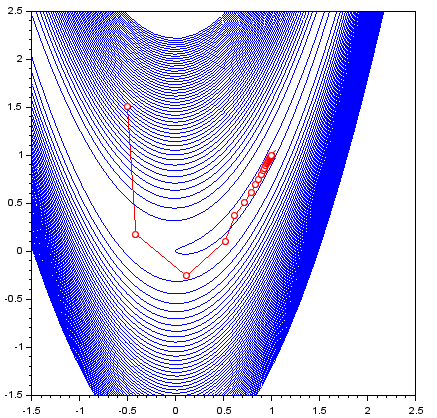
\includegraphics[width=0.6\textwidth]{images/LM1.png}
              \caption{Méthode de Levenberg-Marquardt appliqué à la fonction de Rosenbrock}
              \label{fig:LM1}
            \end{figure}
            \\
            On peut maintenant tester le programme pour des valeurs différentes de $\lambda$. On obtient alors les figures suivantes:
            \newpage
            \begin{figure}[H]
              \centering
              \captionsetup{font=small}
                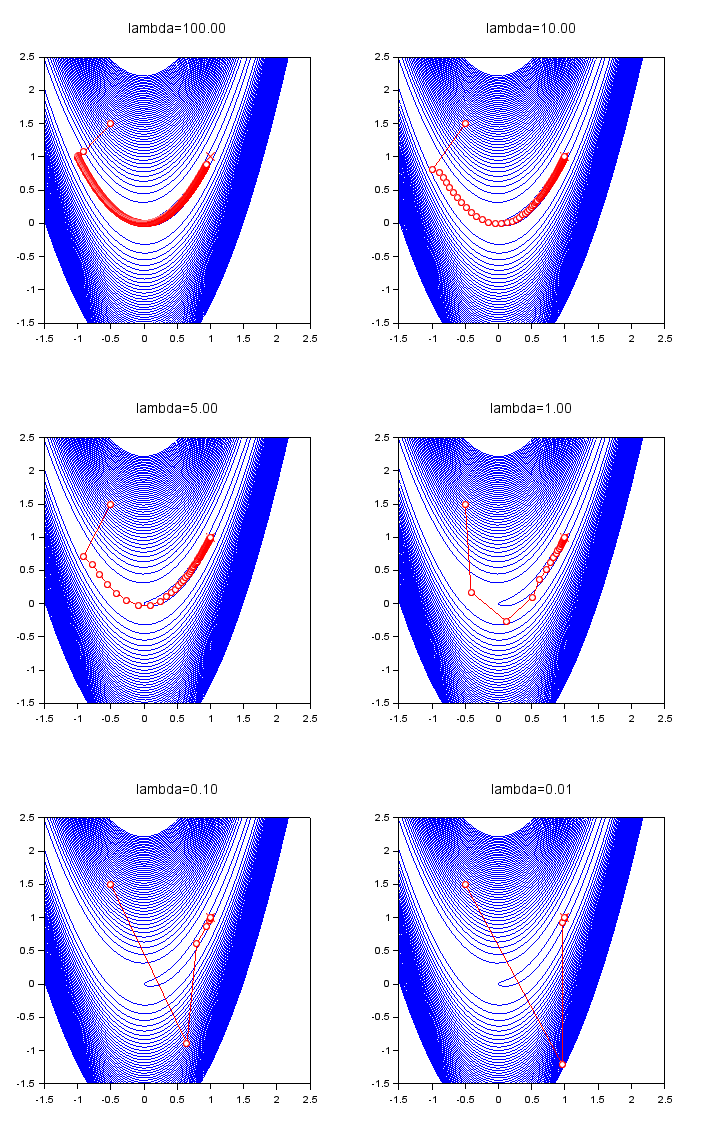
\includegraphics[width=0.85\textwidth]{images/LM2.png}
              \caption{Méthode de Levenberg-Marquardt appliqué à la fonction de Rosenbrock pour des valeurs de $\lambda$ différentes}
              \label{fig:LM2}
            \end{figure}
            A travers ces représentations, on observe que plus $\lambda$ a une valeur élevée, plus le programme doit effectuer d'opérations rendant la convergence vers le minimum très lente. A l'inverse, plus la valeur de $\lambda$ diminue, plus le temps d'exécution est court avec un nombre d'itérations bas. A partir d'un $\lambda$ trop faible, la convergente devient incohérente car les points intermédiaires s'éloignent trop des courbes iso-valeurs. \\A priori, une valeur optimale de lambda se trouverait entre 1 et 0.1. 
            Finalement, c'est le fait que $\lambda$ soit un méta-paramètre qui fait de la méthode Levenberg-Marquardt une méthode intéressante.
            \\\\
            On peut aussi remarquer avec cette méthode, qu'en partant de cette expression 
            $$
            x_{k+1} = x_k - [r'(x_k)^Tr'(x_k)+\lambda I]^{-1}r'(x_k)^Tr(x_k),
            $$
            On peut écrire
            $$
            x_{k+1} = x_k - \frac{1}{2\lambda}\left [\frac{1}{\lambda}r'(x_k)^Tr'(x_k)+I\right ]^{-1}\nabla f(x_k),
            $$
            et lorsque $\lambda$ est grand, la méthode se comporte alors comme la méthode du gradient avec un paramètre donné.\\\\
            De la même manière, la méthode du gradient permet de trouver le minimum d'une fonction $f(x)$, selon la méthode itérative définie par : 
            $$
            x_{k+1} = x_k - p\nabla f(x_k), p>0
            $$
            Pour notre exemple avec la fonction de Rosenbrock, on peut également y appliquer cette méthode pour trouver le minimum.\\ L'idée de la méthode du gradient est, à chaque itération, de se "déplacer" dans la direction opposée au gradient. Une valeur de p plus élevé permettra une rapidité accrue tandis qu'une valeur de p plus faible conduira à une meilleur précision. \\Cependant, une valeur trop élevée risquerait de créer un comportement oscillatoire autour du minimum. A l'inverse, une valeur trop faible allongera énormément le temps d'exécution et pourra rester "bloquée" dans un minimum local produisant un résultat biaisé.
            \\\\Pour notre exemple avec la fonction de Rosenbrock,
            on a 
            $$
            \nabla f(x) = \begin{pmatrix}
                -2(1-x_{1}-400x_1(x_2-x_1^2)\\
                200(x_2-x_1^2)
            \end{pmatrix}
            $$
            L'implémentation dans Scilab peut se faire ainsi :
            \begin{center}
          \begin{minted}[escapeinside=||,mathescape=true,breaklines, breakafter=-\{\}\%+-*]{scilab}
function g=grad(x)
    g = [-2*(1-x(1))-400*x(1)*(x(2)-x(1)^2)
         200*(x(2)-x(1)^2)];
endfunction
clf;
t=linspace(0,2*%pi,1000);
isoview ;
plot(1,1,'xr');
x=[-0.5;1.5];
plot(x(1),x(2),'or');
for k=1:100
    x=x-0.002*grad(x);
    plot(x(1),x(2),'or');
end
          \end{minted}
                \captionof{listing}{Méthode du gradient sur la fonction de Rosenbrock}
                \label{lst:code_13}
         \end{center}
         La valeur du gradient étant très élevée par rapport au domaine étudié, il est nécessaire d'avoir une valeur de $p$ de cette ordre pour obtenir un résultat satisfaisant. Voici la représentation obtenue :
         \newpage
         \begin{figure}[H]
              \centering
                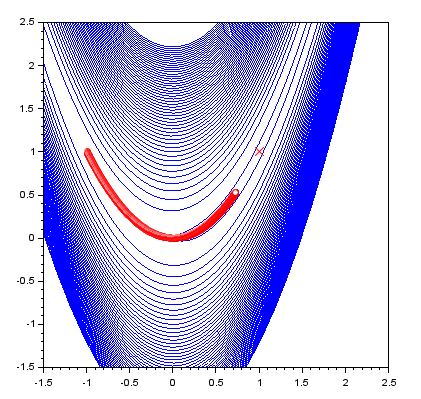
\includegraphics[width=0.6\textwidth]{images/gradient.png}
              \caption{Méthode du gradient appliqué à la fonction de Rosenbrock}
              \label{fig:grad1}
            \end{figure}
            Concrètement, dans les logiciels et les techniques actuels, que ce soit pour des méthodes similaires à Levenberg-Marquardt ou celle du gradient, les valeurs de $\lambda$ ou du paramètre $p$ varient à chaque itération pour obtenir de meilleurs résultats. Cette variation se fait, par exemple, automatiquement dans les macros Scilab prévues à cet effet que nous allons utiliser dans la section suivante.
      \subsubsection{Problèmes de régression non-linéaire}
      La méthode de Levenberg-Marquardt permet de résoudre des problèmes de régression non-linéaires dont nous allons étudier un exemple maintenant. On considère un jeu de données $(t_i,y_i)_{i=1...n}$ que l'on souhaite approcher par une gaussienne de fonction 
      $$
      f(t) = a \exp(\frac{-(t-\mu)^2}{\sigma^2}).
      $$
      On cherche à minimiser 
      $$
      E(a,\mu,\sigma) = \sum^n_{i=1}(f(t_i)-y_i)^2 = \lVert r(\theta)\lVert^2.
      $$
      On a donc 
      $$
      r(\theta) = \begin{pmatrix}
          f(t_1)-y_1\\\vdots\\f(t_n)-y_n
      \end{pmatrix}
      $$
      La jacobienne s'écrit 
      $$
      r'(\theta) = \begin{pmatrix}
          \frac{\partial f(t_1)}{\partial a}&\frac{\partial f(t_1)}{\partial \mu}&\frac{\partial f(t_1)}{\partial \sigma}\\
          \vdots&\vdots&\vdots\\
          \frac{\partial f(t_n)}{\partial a}&\frac{\partial f(t_n)}{\partial \mu}&\frac{\partial f(t_n)}{\partial \sigma}
      \end{pmatrix},
      $$
      avec 
      \begin{align*}
          &\frac{\partial f(t)}{\partial a} = \exp(\frac{-(t-\mu)^2}{\sigma^2})\\
          &\frac{\partial f(t)}{\partial a} = a\exp(\frac{-(t-\mu)^2}{\sigma^2})\times \frac{2}{\sigma^2}(t-\mu)\\
          &\frac{\partial f(t)}{\partial a} = a\exp(\frac{-(t-\mu)^2}{\sigma^2})\times \frac{2}{\sigma^3}(t-\mu)^2
      \end{align*}
      On utilise notre implémentation de Levenberg-Marquardt pour résoudre ce problème de régression sur Scilab :
       \begin{center}
          \begin{minted}[escapeinside=||,mathescape=true,breaklines, breakafter=-\{\}\%+-*]{scilab}
load dataGaussian.sod; //chargement du jeu de donnée à approcher
function [r,rprime] =resid(theta)
    a=theta(1);
    mu = theta(2);
    sigma = theta(3);
    e = exp(-(t-mu).^2/sigma^2) //évite de devoir effectuer plusieurs fois ce calcul
    r = a*e-y;
    rprime = [e,2*a*e.*(t-mu)/sigma^2, 2*a*e.*(t-mu).^2/sigma^3]
endfunction
theta = [0;0;1];
lambda = 1
TOL = 1e-6;
for k=1:2000
    thetap = theta;
    [r,rprime] = resid(theta);
    theta=theta-[rprime; sqrt(lambda)*eye(3,3)]\[r; zeros(3,1)];
    if (norm(thetap-theta) < TOL)
        break;
    end
end
t2=linspace(-4,10,100);
a=theta(1);
mu = theta(2);
sigma = theta(3);
plot(t2,a*exp(-(t2-mu).^2/sigma^2),'r','thickness',2);
plot(t,y,'o');
          \end{minted}
                \captionof{listing}{Régression non linéaire avec la méthode de Levenberg-Marquardt}
                \label{lst:code_14}
         \end{center}
      En représentant à l'écran les points du jeu de données initial et la gaussienne obtenue grâce aux paramètres trouvés on obtient la figure suivante :
      \begin{figure}[H]
              \centering
                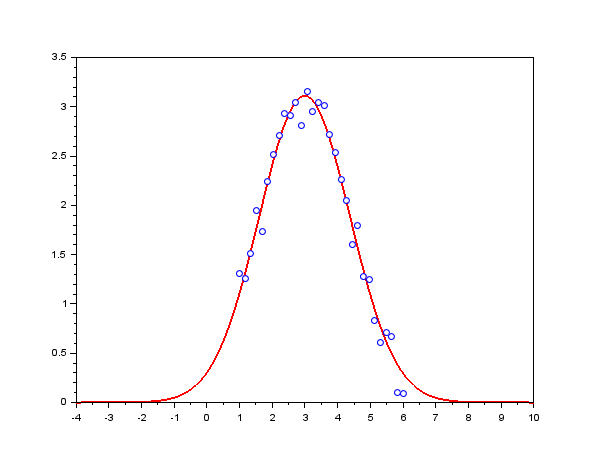
\includegraphics[width=0.8\textwidth]{images/reg_non_lin.png}
              \caption{Représentation graphique de la gaussienne obtenue par résolution d'un problème de régression non linéaire par la méthode de Levenberg-Marquardt}
              \label{fig:renl1}
            \end{figure}
   Ce problème de régression peut aussi se résoudre grâce à la macro Scilab lsqrsolve utilisant une méthode similaire à celle de Levenberg-Marquardt qui peut également approximer la jacobienne du résidu. On l'utiliserait de cette manière sur Scilab :
   \begin{center}
          \begin{minted}[escapeinside=||,mathescape=true,breaklines, breakafter=-\{\}\%+-*]{scilab}
load dataGaussian.sod;
function r=resid(theta,n)
    r = theta(1)*exp(-(t-theta(2)).^2/theta(3)^2)-y;
endfunction
theta0 = [0;0;1];
theta = lsqrsolve(theta0,resid,length(y)); // on aurait pu fournir en paramètre la fonction permettant de calculer la jacobienne pour éviter du temps de calcul
t2=linspace(-4,10,100);
a=theta(1);
mu = theta(2);
sigma = theta(3);
clf;
plot(t2,a*exp(-(t2-mu).^2/sigma^2),'r','thickness',2);
plot(t,y,'o');
          \end{minted}
                \captionof{listing}{Régression non linéaire avec lsqrsolve}
                \label{lst:code_15}
         \end{center}
    \subsection{Applications à un réseau de neurone}
    Pour résoudre des problèmes de régression linéaire, il peut également être intéressant d'utiliser une autre approche, qui ne demande pas la même préparation au préalable et qui peut fonctionner pour tous types de données à approximer : les réseaux de neurones.\\\\
    En informatique, ils sont caractérisés par un ensemble de noeuds inter-connectés dotés d'entrées et de sorties. Les plus connus sont les réseaux de neurone à propagation avant et ce sont ceux que nous allons étudier par la suite. Ils se caractérisent par une propagation acyclique en leur sein.\\\\
    Le plus simple d'entre eux mais aussi le plus ancien est le perceptron, inventé en 1957 par le neurobiologiste/informaticien américain Frank Rosenblatt.
    \subsubsection{Un perceptron pour résoudre un problème de régression linéaire}
    Concrètement, un perceptron est un algorithme d'apprentissage supervisé ayant le rôle d'un classifieur binaire, c'est à dire un algorithme qui permet de diviser un ensemble en deux groupes selon des propriétés similaires. A partir de cette première approche, on comprend dès à présent son intérêt pour traiter des régressions linéaires dans un premier temps. Pour comprendre son fonctionnement voici un schéma décrivant son architecture : 
    \begin{figure}[H]
              \centering
                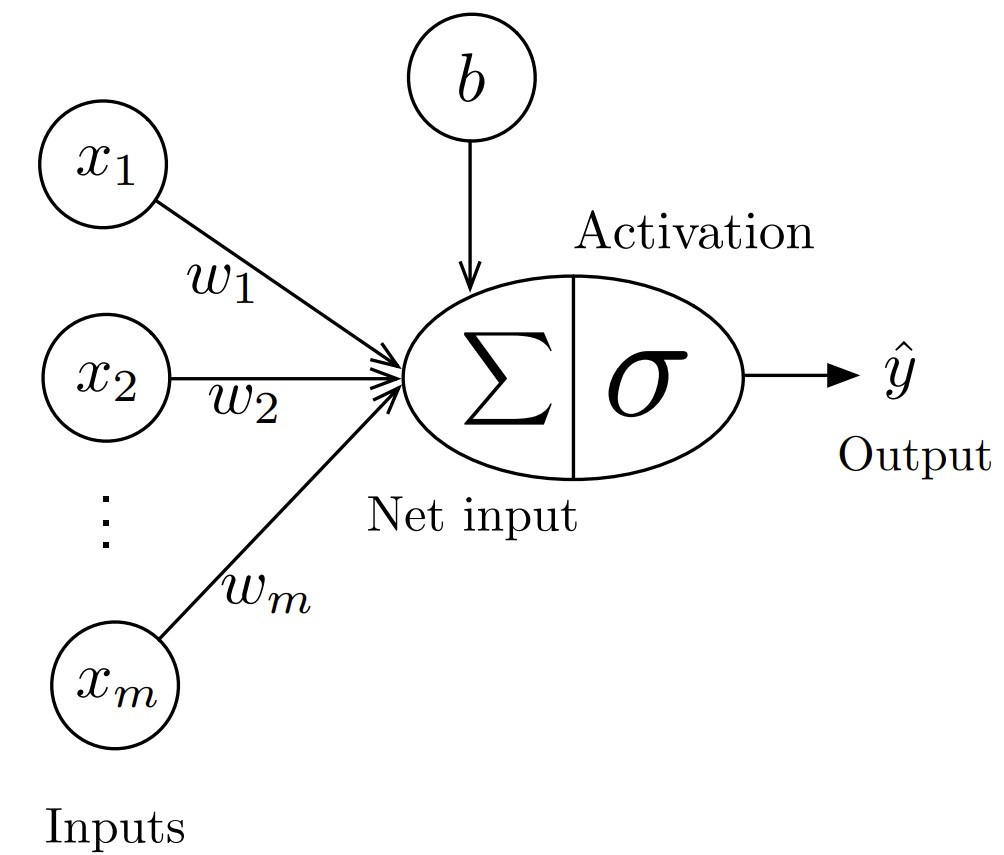
\includegraphics[width=0.7\textwidth]{images/perceptron.jpg}
              \caption{Schéma d'un perceptron}
              \label{fig:rn1}
            \end{figure}

    Un perceptron prends en entré un ensemble de valeurs $(x_i)_{i\in \llbracket 1, m \rrbracket}$ puis l'entrée nette constitue la combinaison linéaire des entrées par leur poids associé additionné à un biais $b$: 
    $$
    b + \sum^N_{i=1} x_iw_i
    $$
    Ensuite, le neurone est caractérisé par une fonction d'activation qui peut prendre différente formes en fonction de ce que l'on veut obtenir : fonction de seuil, sigmoïde, fonction Rectified Linear Unit (ReLU) caractérisée par x si x supérieur à 0, 0 sinon, ou encore une fonction linéaire.\\
    Dans le cas d'une régression linéaire classique on utilisera une fonction d'activation linéaire. Finalement, on a
    $$
    y=f(b + \sum^N_{i=1} x_iw_i)=b + \sum^N_{i=1} x_iw_i.
    $$
    Cependant, à partir de cela, il est impossible d'obtenir quoi que ce soit. Tout le problème et la majeur partie du temps de calcul de l'algorithme va être l'entraînement afin de trouver les poids les plus adaptés pour résoudre le problème.\\Une méthode naïve consisterait à choisir aléatoirement des poids, puis à tester les valeurs obtenus en calculant l'erreur associée. Cette méthode serait évidemment beaucoup trop longue et pas du tout efficace. C'est pour cette raison qu'on va utiliser la méthode de descente du gradient pour faire varier les poids dans la direction opposée au gradient afin d'atteindre le minimum qui nous intéresse (méthode survolée dans \hyperref[subsubsec:LM]{cette} partie). La méthode que nous allons utilisée est l'algorithme du gradient stochastique qui est une méthode de descente de gradient itérative pour minimiser une fonction objectif, ici, notre erreur.
    \\\\
    Soit $(x_i,y_i)$ notre dataset à approximer par une droite. Notre objectif ici va être avec un perceptron d'une seul entrée x d'obtenir sa sortie selon le modèle $ax+b$ avec le poids $a$ et le biais $b$. On défini alors un vecteur paramètres $$
    w = \begin{bmatrix}
        a\\b
    \end{bmatrix}
    $$
    et un vecteur prédiction 
    $$
    P = Xw = \begin{bmatrix}
        x_1&1\\\vdots&\vdots\\x_n&1
    \end{bmatrix}\begin{bmatrix}
        a\\b
    \end{bmatrix}=\begin{bmatrix}
        ax_1+b\\\vdots\\ax_n+b
    \end{bmatrix}
    $$
    avec $X$ la matrice composée d'une première colonne composée des entrées $x_i$ et une deuxième composée que de 1 pour le biais.\\
    La fonction de coût ou erreur  à minimiser sera l'erreur quadratique moyenne (mean squared error) définie par
    $$
    E(a,b) = \frac{1}{2n}\sum^n_{i=1}(ax_i+b-y_i)^2 =\frac{1}{2n}\sum^n_{i=1}(P-Y)^2
    $$
    avec $Y$ le vecteur des $y_i$. \\
    Pour le calcul de notre gradient on a 
    $$
    \nabla E (a,b)= \begin{bmatrix}
        \frac{\partial E(a,b)}{\partial a}\\\frac{\partial E(a,b)}{\partial b}
    \end{bmatrix}
    $$
    avec 
    \begin{align*}
        &\frac{\partial E(a,b)}{\partial a} = \frac{1}{n}\sum^m_{i=1}x_i(ax_i+b-y_i)\\
        &\frac{\partial E(a,b)}{\partial b} = \frac{1}{m}\sum^m_{i=1}(ax_i+b-y_i)
    \end{align*}
    On peut vectoriser ces expressions ainsi
    $$
    \nabla E(a,b) = \frac{1}{m} X^T(P-Y)
    $$

    Enfin, la mise à jour des poids et biais à chaque itération se fera selon la formule 
    $$
    w = w - \alpha \nabla E(a,b)
    $$
    avec $\alpha$ la valeur du learning rate qu'on fixera à 0.01 dans notre exemple pour obtenir des valeurs cohérentes.\\
    Dans Scilab, tous ces éléments peuvent se concrétiser avec le programme suivant :
    \begin{center}
          \begin{minted}[escapeinside=||,mathescape=true,breaklines, breakafter=-\{\}\%+-*]{scilab}
//création du dataset
clf;
n=1000;
t=linspace(0,20,n)';
rand('seed',1);
y=t+rand(n,1,'normal').*2+5;//ajout de bruit
plot(t,y,'o');
//initialisation des variables
t= [t, ones(n,1)];
learning_rate = 0.01; //taux d'apprentissage
max_iterations = 100 ; //nombre maximal d'itérations
err=[];
w = rand(2,1,'normal') //poids et biais aléatoires
//entrainement
for i = 1:max_iterations
    //prédiction de la sortie
    y_pred = t*w;
    err = [err norm(y_pred-y)];
    grad = (1/n)*t'*(y_pred-y);
    //mise à jour des poids
    w = w - learning_rate * grad;
end
plot(t, w(1)*t+w(2),'r','thickness',3);
//on peut tracer l'erreur ensuite
          \end{minted}
                \captionof{listing}{Perceptron simple pour résoudre un problème de régression linéaire utilisant une descente de gradient pour l'apprentissage}
                \label{lst:code_16}
         \end{center}
         A partir de ce code on peut résoudre n'importe quelle problème de régression linéaire à partir d'un jeu de données.
         \\Le code en particulier permet d'obtenir cette figure : 
         \begin{figure}[H]
              \centering
                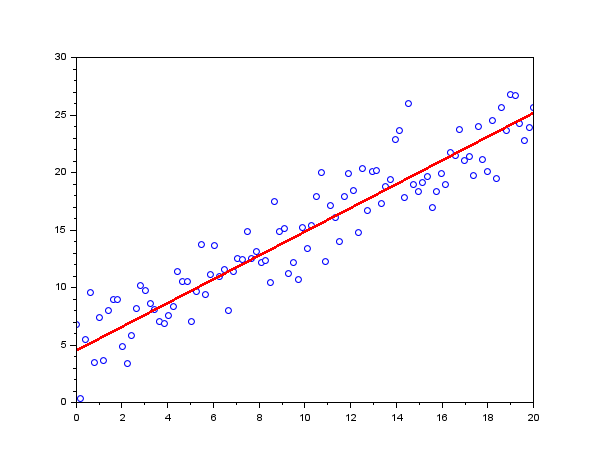
\includegraphics[width=0.7\textwidth]{images/perceptron_lineaire.png}
              \caption{Régression linéaire obtenue à partir de l'entraînement d'un perceptron}
              \label{fig:rn2}
            \end{figure}
            Le résultat semble correspondre aux données du dataset, cependant, en augmentant le nombre d'itération on aura un résultat à priori meilleur.
            Traçons l'erreur pour 10000 itérations :
            \begin{figure}[H]
              \centering
                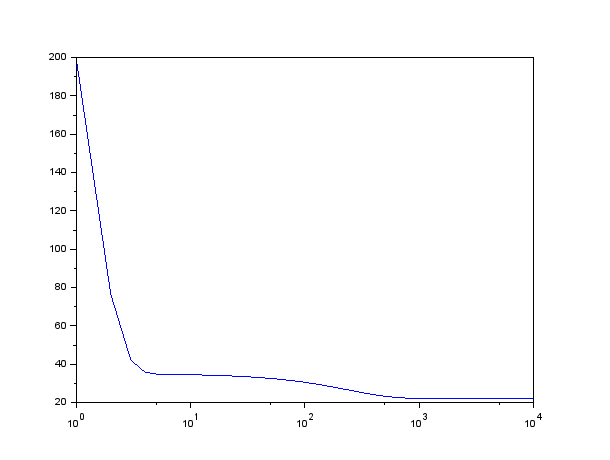
\includegraphics[width=0.7\textwidth]{images/perceptron_lineaire_erreur.png}
              \caption{Erreur de la régression linéaire obtenue à partir de l'entraînement d'un perceptron}
              \label{fig:rn3}
            \end{figure}
        On observe que l'erreur diminue très vite initialement, ce qui est logique car les paramètres étaient pris aléatoirement, puis qu'elle devient "acceptable" à partir de 1000 itérations ce qui nous permet d'avoir un résultat rapide et efficace. En effet, l'erreur obtenue à la 1000ème itération est de $22.08$ dans notre exemple contre $21.97$ pour la 10000ème. Le gain de précision obtenue avec des itérations supérieures à 1000 n'est pas intéressant par rapport au temps perdu.
        \subsubsection{Un réseau neuronale multicouche pour des problèmes plus compliqués}
        Maintenant qu'on a vu comment résoudre un exemple simple de régression, nous allons nous intéresser aux perceptrons multicouche, qui sont, en fait, des réseaux neuronales à plusieurs couches : l'entrée, la sortie et les/la couche cachées. Notre objectif va être de résoudre des problèmes de régressions quelconques en utilisant un réseaux de neurones à une seule couche cachée.\\
        L'architecture de notre réseaux suivra le principe du schéma suivant (le nombre de neurones par couche/d'entrées sera différent) : 
        \begin{figure}[H]
              \centering
                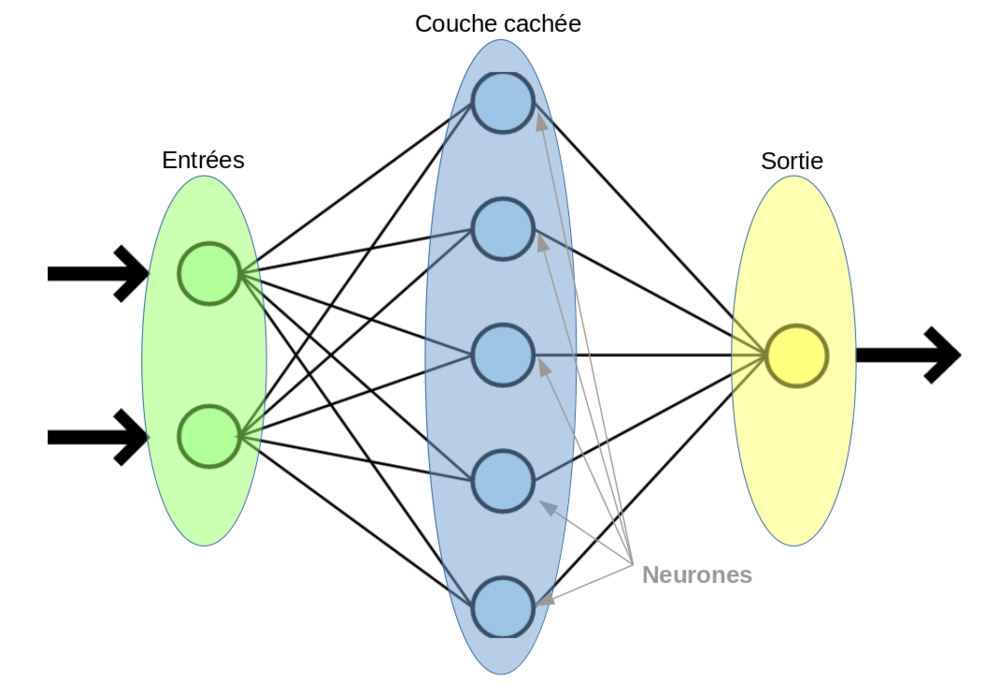
\includegraphics[width=0.7\textwidth]{images/rdn.png}
              \caption{Schéma réseau de neurones multicouche}
              \label{fig:rn4}
            \end{figure}
        Dans ce type de réseau, il y aura 2 fonctions d'activation : la fonction d'activation des noeuds cachés $f(x) = \sigma(x) = 1/(1+\text{e}^{-x})$ qui sera une sigmoïde et la fonction d'activation de sortie $f_{\text{sortie}}(x) = x$ qui sera l'identité.\\
        Le principe sera similaire à ce qui a été fait précédemment, en utilisant la descente de gradient, on va adapter les poids et biais entre chacun des noeuds. En utilisant un learning rate $\alpha$. On utilisera un dataset composé des couples $(x_i,y_i)_{i\in \llbracket1,n\rrbracket}$.
        L'erreur calculé sera toujours l'erreur quadratique moyenne.
        $$
        E(\theta) = \frac{1}{2n}\sum^n_{i=1}(\hat{y}_i-y_i)^2
        $$
        avec $\theta$ représentant les paramètres et $\hat{y_i}$ la sortie calculée par le réseau pour l'entrée $x_i$.
        \\\\
        Le problème principal des réseaux de neurones avec une couche cachée qui, contrairement aux perceptrons simples, ont une règle pour approximer une sortie cible bien définie, est que les noeuds des couches cachées n'ont pas de sortie cible car ils sont utilisés comme étapes intermédiaires dans le calcul. On ne peut donc pas définir une fonction d'erreur spécifique à un noeud caché car toute fonction d'erreur pour ce noeud dépendra des valeurs des paramètres des couches précédentes (qui déterminent l'entrée du noeud) et des couches suivantes (car la sortie affectera le calcul de la fonction d'erreur $E(\theta)$. Ce couplage des paramètres du réseau rend les calculs assez compliqués, ce qui peut ralentir les calculs finaux s'ils ne sont pas effectuer intelligemment. Nous utiliserons alors la méthode de la rétropropagation du gradient pour simplifier les calculs de la descente de gradient. \\
        Dans notre exemple, on notera $w^k_{ij}$ le poids pour le noeud j de la couche $k$ pour le noeud entrant $i$, $b^k_i$ le bais pour le noeud $i$ de la couche $k$, $a_i^k$ la somme des produit des entrées du noeud ($i$ de la couche $k$) par les poids, plus le biais, $o^k_i$ la sortie du noeud $i$ de la couche $k$ et enfin $r_k$, le nombre de noeuds dans la couche k.
        \\Pour simplifier les calculs, le biais sera incorporé avec les poids de sorte que 
        $$
        a^k_i = b^k_i + \sum^{r_{k-1}}_{j=1}w^k_{ji}o^{k-1}_j = \sum^{r_{k-1}}_{j=0}w^k_{ji}o^{k-1}_j
        $$
        On a donc fixé
        $$
        w^k_{0i} = b^k_i
        $$
        avec une sortie fixe $o^{k-1}_0 = 1$ pour le noeud 0 de la couche $k-1$.\\
        La rétropropagation cherche à minimiser la fonction erreur $E(\theta)$ définie plus tôt en calculant ses dérivés partiels $\frac{\partial E(\theta)}{\partial w^k_{ji}}$ pour chacun des poids $w^k_{ji}$.
        \\Par opérations sur les dérivées on peut simplifier le calcul de cette manière :
        \begin{equation}
        \frac{\partial E(\theta)}{\partial w^k_{ij}} = \frac{1}{n}\sum^n_{d=1}\frac{\partial}{\partial w_{ij}^k}\left(\frac{1}{2}(\hat{y_d}-y_d)^2\right) = \frac{1}{n}\sum^n_{d=1}\frac{\partial E_d}{\partial w_{ij}^k}
        \label{eq:formule1}
        \end{equation}
        Pour calculer la dérivé partielle de $E_d$ par rapport à $w^k_{ij}$, on utilisera les règles de dérivés en chaîne
        $$
        \frac{\partial E_d}{\partial w_{ij}^k} = \frac{\partial E_d}{\partial a_{j}^k}\frac{\partial a^k_j}{\partial w_{ij}^k}
        $$
        le premier terme appelé l'erreur sera noté $\delta^k_j$ et le second peut se simplifier ainsi :
        $$
        \frac{\partial a^k_j}{\partial w_{ij}^k} = \frac{\partial}{\partial w_{ij}^k}\left(\sum^{r_{k-1}}_{l=0}w^k_{lj}o^{k-1}_l\right)=o_i^{k-1}
        .$$
        Par conséquent, notre dérivé partielle s'écrit 
        \begin{equation}   
        \frac{\partial E_d}{\partial w_{ij}^k} = \delta^k_jo^{k-1}_i
        \label{eq:formule2}
        \end{equation}
        Il reste toujours à calculer l'erreur $\delta^k_j$ qui dépend de la fonction d'erreur $E_d$. $\delta^k_j$ étant dépendant des valeurs des termes d'erreur de la couche suivante, le calcul des termes d'erreur s'effectuera dans le sens inverse, de la couche de sortie jusqu'à la couche d'entrée d'où le nom "rétropropagation" pour l'algorithme. (nous le verrons mathématiquement ensuite) \\\\
        En partant de la \textbf{couche de sortie}, on cherche à calculer $\delta^m_1$ avec m l'indice de la dernière couche du réseau de neurone ($m$ sera égal à 2 dans notre réseau car la couche d'entrée est d'indice 0). 
        \\Ainsi $$
        E_d = \frac{1}{2}(\hat{y_d}-y_d)^2=\frac{1}{2}(f_{\text{sortie}}(a^m_1)-y_d)^2
        $$
        avec $f_{\text{sortie}}$ la fonction d'activation de sortie qui est l'identité.\\
        Ainsi,
        \begin{equation}
            \delta^m_1 = (f_{\text{sortie}}(a_1^m)-y_d)f'_{\text{sortie}}(a^m_1)
            \label{eq:formule3}
        \end{equation}
        Finalement, pour la couche de sortie, on a :
        $$
        \frac{\partial E_d}{\partial w_{i1}^m} = (f_{\text{sortie}}(a_1^m)-y_d)f'_{\text{sortie}}(a^m_1)o^{m-1}_i
        $$
        Pour notre exemple, comme la fonction d'activation de sortie est l'identité, on peut simplifier $\delta^m_1$ ainsi
        $$\delta^m_1 = a^m_1-y_d = \hat{y_d}-y_d$$
        Maintenant, pour calculer les \textbf{couches cachées}, on utilise encore une fois les dérivées en chaîne : 
        $$
        \delta^k_j = \frac{\partial E_d}{\partial a^k_j} = \sum^{r^{k+1}}_{l=1}\frac{\partial E}{\partial a_l^{k+1}}\frac{\partial a_l^{k+1}}{\partial a_j^{k}}=\sum^{r^{k+1}}_{l=1}\delta^{k+1}_j\frac{\partial a_l^{k+1}}{\partial a_j^{k}}$$
        avec $1\leq k < m$.\\
        \\Comme le biais de l'entrée $o^k_0$ qui correspond à $w^{k+1}_{0j}$ est fixé, sa valeur ne dépend pas des sorties des couches précédentes donc $l$ commence à 1.
        \\On a 
        $$
        a^{k+1}_l = \sum^{r_{k}}_{j=1}w^{k+1}_{jl}o^{k}_j=\sum^{r_{k}}_{j=1}w^{k+1}_{jl}f(a^k_j)
        $$
        avec $f$ la fonction d'activation pour les couches cachées (sigmoïde).\\
        \\
        En dérivant partiellement cette expression par $a^k_j$ et en l'intégrant dans l'expression de $\delta^k_j$, on obtient la formule :
        \begin{equation}
            \delta^k_j = \sum^{r^{k+1}}_{l=1}\delta^{k+1}_jw^{k+1}_{jl}f'(a^k_j)
            \label{eq:formule4}
        \end{equation}
        Ce qui nous donne au final
        $$
        \frac{\partial E_d}{\partial w_{ij}^k} = \delta^k_jo^{k-1}_i=f'(a^k_j)o^{k-1}_i\sum^{r^{k+1}}_{l=1}\delta^{k+1}_jw^{k+1}_{jl}
        $$
        avec $1\leq k < m$.\\\\
        Dans notre cas, $f$ est la fonction sigmoïde et $f'(x)=\sigma '(x) = \sigma (x)(1-\sigma(x))$.
        Ainsi, $$
        \delta^k_j = o^k_j(1-o^k_j)\sum^{r^{k+1}}_{l=1}\delta^{k+1}_jw^{k+1}_{jl}.
        $$
        Le fait que $\delta^k_j$ dépende bien de $\delta^{k+1}_j$ témoigne le fait qu'il est nécessaire de calculer les erreurs de la dernières couches vers celles de la première d'où le terme "rétro" dans le nom de l'algorithme.\\\\
        La modification des poids pour chaque itération s'effectuera par descente de gradient en utilisant la formule pour chacun des paramètres du réseaux de neurones : 
        \begin{equation}
           \hat{w^k_{ij}} = w^k_{ij} - \alpha \frac{\partial E(\theta)}{\partial w^k_{ij}}
           \label{eq:formule5}
        \end{equation}
        avec $\hat{w^k_{ij}}$ la valeur du poids modifiée.
        \\\\
        Globalement, notre algorithme va s'effectuer en 2 grandes phases. La première s'effectuera vers \textbf{l'avant} : l'algorithme va parcourir le réseau neuronale de gauche à droite en effectuant les calculs pour chaque noeud. Ensuite la deuxième phase s'effectuera vers \textbf{l'arrière} (rétropropagation du gradient), consistera à calculer $\frac{\partial E_d}{\partial w_{ij}^k}$ (en utilisant les formules \ref{eq:formule2}, \ref{eq:formule3} et \ref{eq:formule4}) pour chacun des poids $w^k_{ij}$ en partant de la dernière couche $m$ vers la première. Au final, l'algorithme combinera les $\frac{\partial E_d}{\partial w_{ij}^k}$ pour calculer $\frac{\partial E(\theta)}{\partial w^k_{ij}}$ en utilisant la formule \ref{eq:formule1} pour finalement mettre à jour les poids à l'aide de la formule \ref{eq:formule5}.
        \\\\Pour une meilleur optimisation et une exécution rapide dans Scilab, on préférera utiliser des calculs vectoriels et matriciels, ce qui aura pour résultat une exécution simultanée de certains calculs exprimés précédemment. Voici un programme permettant de résoudre des problèmes de régression en Scilab :
        \begin{center}
          \begin{minted}[escapeinside=||,mathescape=true,breaklines, breakafter=-\{\}\%+-*]{scilab}
//insérer un dataset (t,y)
clf;
plot(t,y,'o'); //tracé des points initiales avec lesquels on souhaite effectuer la regression 
function y = sigmoid(x)
    y = 1./(1+exp(-x));
endfunction
//paramètres de l'algorithme
alpha = 0.1; //learning rate
num_hidden = 8; // nombre de noeuds cachés 
num_iterations = 10000; //nombre d'itérations
//initialisation des poids/biais aléatoirement
hidden_weights = rand(2, num_hidden);
output_weights = rand(num_hidden+1, 1);
err = [];
n = size(t, 1); //éviter de refaire le calcul à chaque itération
input_layer_outputs = [ones(n, 1), t];
for i = 1:num_iterations
    //phase avant
    hidden_layer_outputs = [ones(n, 1), sigmoid(input_layer_outputs * hidden_weights)];
    output_layer_outputs = hidden_layer_outputs * output_weights;
    //phase arrière
    output_error = output_layer_outputs - y;//on utilise la formule (3) adaptée pour l'identité
    hidden_error = hidden_layer_outputs(:, 2:$) .* (1 - hidden_layer_outputs(:, 2:$)) .* (output_error * output_weights(2:$, :)');//on utilise la formule (4) appliquée à la fonction sigmoïde
    //calcul des dérivée partielles + du gradient de l'erreur quadratique moyenne
    total_hidden_gradient = input_layer_outputs' * hidden_error / n;
    total_output_gradient = hidden_layer_outputs' * output_error / n;
    //mise à jour des poids
    hidden_weights = hidden_weights - alpha .* total_hidden_gradient;
    output_weights = output_weights - alpha .* total_output_gradient;
    
    err = [err, norm(output_layer_outputs - y)^2];
end
plot(t, output_layer_outputs, 'r', 'thickness', 2);
          \end{minted}
                \captionof{listing}{Réseau neuronale multicouche permettant de résoudre des problèmes de régressions utilisant l'algorithme de rétropropagation du gradient}
                \label{lst:code_17}
         \end{center}
        En utilisant ce programme pour les exemples précédents comme celui avec les données polynomiales, la gaussienne ou d'autre fonction linéaire ou non on peut obtenir les régressions suivantes : 
        \begin{figure}[H]
        \centering
        \begin{minipage}[H]{0.48\textwidth}
            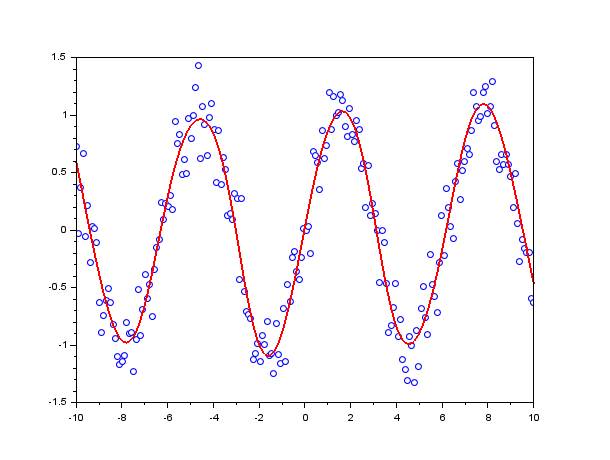
\includegraphics[width=\textwidth]{images/rdn_sin.png}
            \caption{Régression pour la fonction sinus avec un bruit}
        \end{minipage}
        \hfill
        \begin{minipage}[H]{0.48\textwidth}
            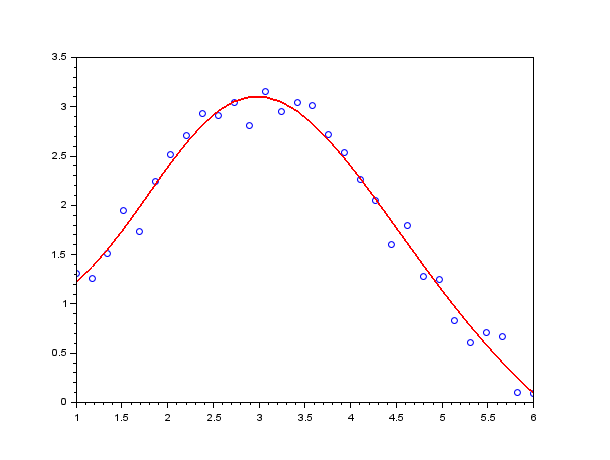
\includegraphics[width=\textwidth]{images/rdn_gauss.png}
            \caption{Régression pour les données utilisées pour la figure \ref{fig:renl1}}
        \end{minipage}
    \end{figure}
    \begin{figure}[H]
        \centering
        \begin{minipage}[H]{0.48\textwidth}
            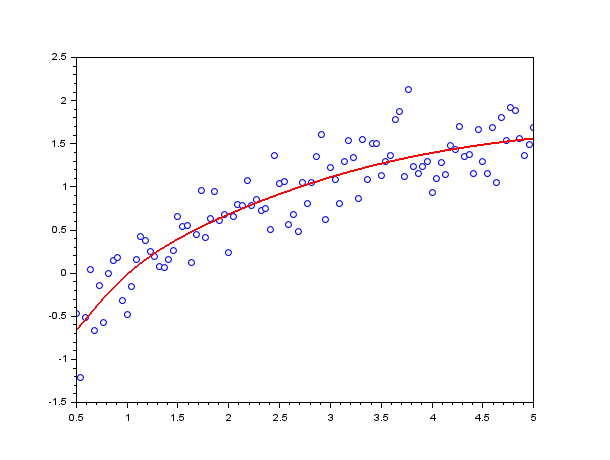
\includegraphics[width=\textwidth]{images/rdn_log.png}
            \caption{Régression pour la fonction logarithme avec un bruit}
        \end{minipage}
        \hfill
        \begin{minipage}[H]{0.48\textwidth}
            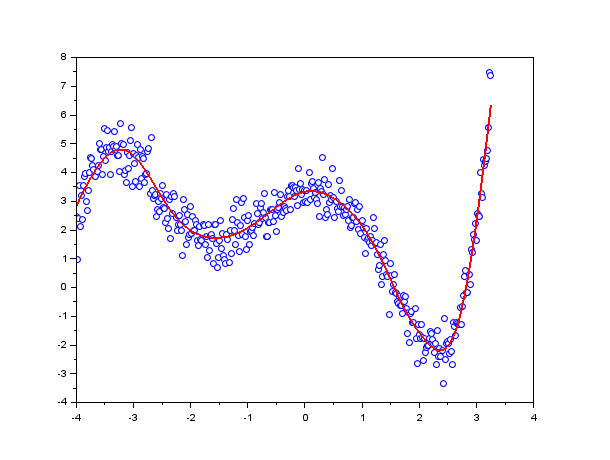
\includegraphics[width=\textwidth]{images/rdn_poly.png}
            \caption{Régression issue des données utilisées au code source \ref{lst:code_6}}
        \end{minipage}
    \end{figure}
    Si on trace l'erreur pour la figure 32, pour $10^5$ itérations et 8 noeuds dans la couche cachée, on obtient ce graphique : 
    \begin{figure}[H]
              \centering
                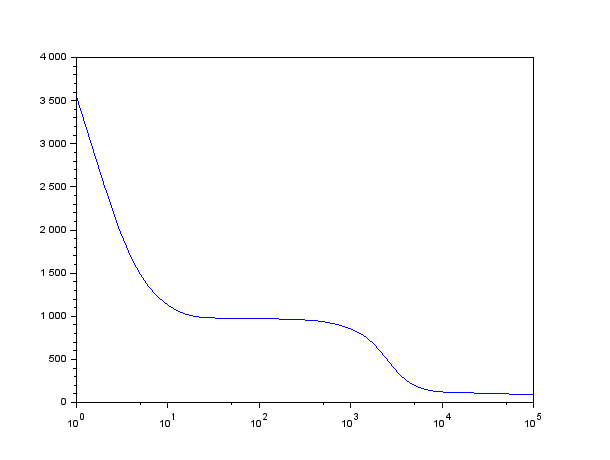
\includegraphics[width=0.7\textwidth]{images/rdn_poly_err.png}
              \caption{Erreur obtenue en fonction du nombre d'itération du réseau de neurones pour 8 noeuds cachés avec le dataset de la figure 32}
              \label{fig:rn2}
            \end{figure}
        On remarque ici, qu'à partir d'environ $10^4$ itérations sur le programme, l'erreur devient similaire à celle obtenue dans le meilleur des cas avec le code source \ref{lst:code_7}. Cependant, le temps d'exécution est plus long (11.7 secondes pour les $10^5$ itérations et ainsi obtenir une erreur minimale de 95.07 contre 92.86 pour le programme classique pour la régression polynomiale). L'avantage de cette méthode est qu'elle fonctionne pour tous types de données relativement rapidemment et avec une précision donc un temps d'exécution facilement interchangeable (aumenter/diminuer le nombre de noeuds cachés, augmenter/diminuer le nombre d'itération).\\\\
        J'ai choisi d'utiliser le réseau de neurones pour des problèmes de régression pour ne pas trop s'écarter du cadre de l'UV MT94 mais avec le principe que j'ai pu détailler dans cette section, et en adaptant l'algorithme utilisé, il est possible de l'appliquer dans de nombreux contexte assez facilement ce qui le rend très intéressant. Bien évidemment, pour des applications plus complexes, il faudra adapter le réseau neuronales avec des méthodes plus avancées, mais le principe initial restera similaire.
        \newpage
   \section*{Valeurs et vecteurs propres}
   \phantomsection
   \markboth{Valeurs et vecteurs propres}{}
   Le calcul des valeurs propres est très souvent utilisé, notamment pour diagonaliser des matrices. Cependant, le calcul exacte de celles-ci peut rapidement devenir long et fastidieux à mesure que le nombre d'élément des matrices augmente. C'est pourquoi, il peut être intéressant d'utiliser des méthodes numériques afin de les approximer de manière bien plus rapide.
    \addcontentsline{toc}{section}{Valeurs et vecteurs propres}
      \subsection{Méthodes des puissances}
      Pour approximer les valeurs propres d'une matrice, il est intéressant d'utiliser les méthodes de la puissance et de la puissance inverse.
      \subsubsection{La méthode de la puissance}
      Cette méthode va itérer de manière successive en se fondant sur le théorème suivant:
      \begin{theoreme}
      Soit A une matrice réelle $n\times n$, diagonalisable et de valeurs propres $(\lambda_i)_{i=\llbracket1,n\rrbracket}$ avec $|\lambda_1|>|\lambda_2|\geq...|\lambda_n|$ et $(y_i)_{i=\llbracket1,n\rrbracket}$ les vecteurs propres associés, tels que $||y_i||=1$.\\
      Soit $x_0\notin Vect(y_2,...,y_n).$ La suite $(x_k)$ définie par $$x_{k+1}=\frac{Ax_k}{||Ax_k||},$$
      converge dans le sous espace propre associé à $y_1$ au sens où
      $$\lim\limits_{k\to +\infty}\text{signe}(\lambda_1)^kx_k=\pm y_1.$$
      \end{theoreme}
      En utilisant la norme Euclidienne on remarque,
      $$
      \lim\limits_{k\to +\infty} x_k^TAx_k=y_1^TAy_1=\lambda_1y_1^Ty_1=\lambda_1||y_1||^2=\lambda_1.
      $$
      On fixe alors une tolérance TOL pour effectuer le test suivant et terminer les itérations de l'algorithme :
      $$
      ||Ax_k-(x_k^TAx_k)x_k||<TOL
      $$
      Dans Scilab j'ai réalisé le code suivant afin d'appliquer cette méthode :
      \begin{center}
          \begin{minted}[escapeinside=||,mathescape=true,breaklines, breakafter=-\{\}\%+-*]{scilab}
//on note A la matrice à étudier
TOL=1e-6;
it_max=1e4;
X=rand(n,1); //avec n le nombre de colonne de A
for i=1:it_max
    mult = A*X;
    mu = X' * mult;
    if norm(mult-mu*X) < TOL
        break;
    end
    X = mult/norm(mult);
end
disp(X);//affiche le vecteur propre associé à lambda1
disp(i);//affiche le nombre d'itération effectué
disp(mu);//affiche la valeur de l'approximation de la valeur propre lambda1
          \end{minted}
                \captionof{listing}{Méthode de la puissance sur Scilab}
                \label{lst:code_18}
         \end{center}
         A la fin du programme, "mu" contient l'approximation de la valeur propre $\lambda_1$ de la matrice $A$. Ce programme est efficace puisqu'en le testant avec une matrice carré de dimension 2 respectant les conditions nécessaires, le programme effectuait entre 10 et 12 itérations. En comparant les résultats avec la macro Scilab "spec", l'erreur était négligeable compte tenu de la précision machine.
      \subsubsection{La méthode de la puissance inverse}
      De manière similaire à la méthode de la puissance, la méthode itérative de la puissance inverse repose sur le théorème suivant : 
      \begin{theoreme}
      Soit A une matrice réelle $n\times n$, diagonalisable et de valeurs propres $(\lambda_i)_{i=\llbracket1,n\rrbracket}$ avec $|\lambda_1|\geq|\lambda_2|\geq...|\lambda_{n-1}|>|\lambda_n|$ et $(y_i)_{i=\llbracket1,n\rrbracket}$ les vecteurs propres associés, tels que $||y_i||=1$.\\
      Soit $x_0\notin Vect(y_1,...,y_{n-1}).$ Si on note $z_k$ la solution du système linéaire $Az_k=x_k,$la suite $(x_k)$ définie par 
      $$x_{k+1}=\frac{z_k}{||z_k||},$$
      converge dans le sous espace propre associé à $y_n$ au sens où
      $$\lim\limits_{k\to +\infty}\text{signe}(\lambda_n)^kx_k=\pm y_n.$$
      \end{theoreme}
      La méthode de la puissance inverse permet de déterminer $\frac{1}{\lambda_n}$ et $y_n$ le vecteur propre associé à $\lambda_n$.\\
      Dans Scilab, cette méthode peut être implémentée de cette façon : 
      \begin{center}
          \begin{minted}[escapeinside=||,mathescape=true,breaklines, breakafter=-\{\}\%+-*]{scilab}
//on note A la matrice à étudier
TOL=1e-6;
it_max=1e4;
X=rand(n,1); //avec n le nombre de colonne de A
for i=1:it_max
    mult = A\X;
    mu = X' * mult;
    if norm(mult-mu*X) < TOL
        break;
    end
    X = mult/norm(mult);
end
disp(X);//affiche le vecteur propre associé à lambda_n
disp(i);//affiche le nombre d'itération effectué
disp(1/mu);//affiche la valeur de l'approximation de la valeur propre lambda_n
          \end{minted}
                \captionof{listing}{Méthode de la puissance inverse sur Scilab}
                \label{lst:code_19}
         \end{center}
         Avec la même matrice et les mêmes paramètres que ceux que j'avais utilisé avec la méthode précédente, les résultats sont aussi satisfaisants. Cependant, le nombre d'itération est en moyenne 2 fois inférieur et, l'erreur avec les résultats obtenus à l'aide de la macro "spec" est supérieure, de l'ordre de $10^{-8}$.
         \newpage
      \subsection{Page Rank}
        La multinationale Google, devenue célèbre initialement grâce à son moteur de recherche, battant toute concurrence en terme d'efficacité, a pu gagner cette renommée grâce à l'algorithme  PageRank, présenté pour la première fois en 1998, s'inspirant du Science Citation Index (SCI), fondé par Eugène Garfield en 1964, qui permettait de classer les article en fonction du nombre de citations qu'ils recevaient. Bien que c'est algorithme a été amélioré depuis est est couplé à de nombreuses autre méthode, nottament d'IA, il est intéressant de s'y interroger pour comprendre son lien avec la section actuelle.\\\\
        Le principe du PageRank est donc de mesurer la pertinence des pages Web en leur attribuant un score qui permettra ensuite de les classer lors d'une recherche de mots clés. Concrètement, il s'appuie sur les hyperliens qui sont des liens vers d'autres pages Web présents sur une page donné. Ainsi, plus une page est référencée (par des pages elles-mêmes pertinentes), plus son rank sera important et donc elle apparaîtra de manière plus prioritaire.
        \begin{figure}[H]
              \centering
                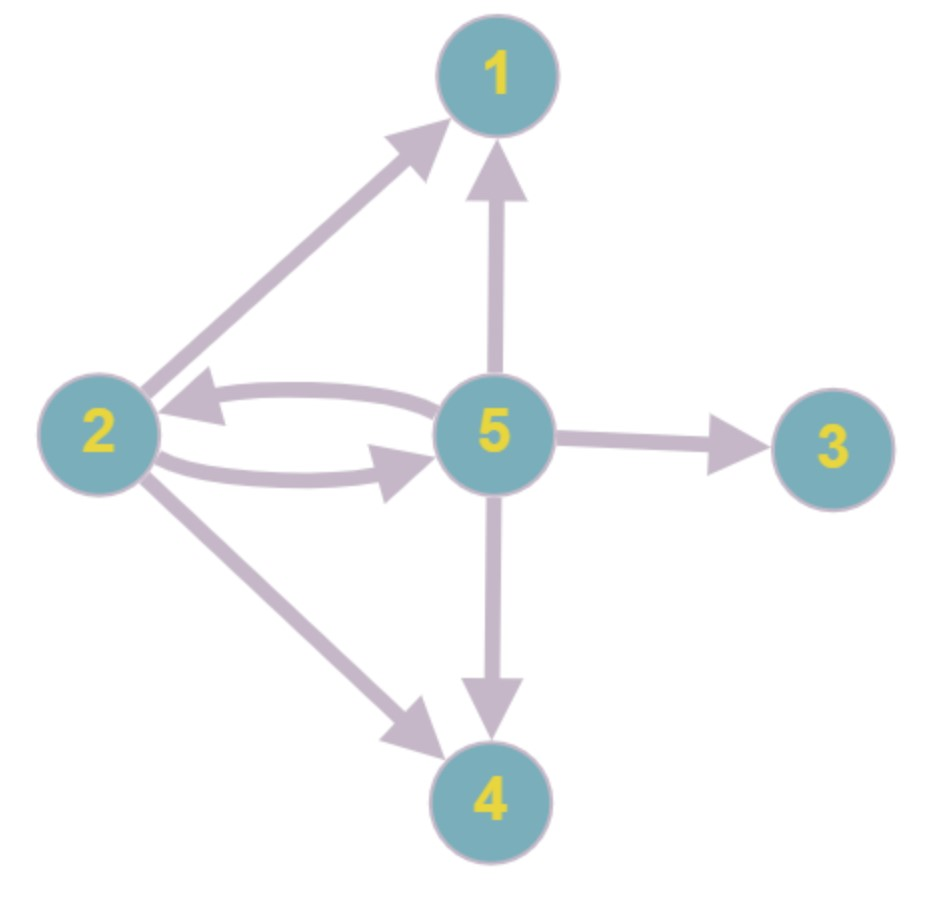
\includegraphics[width=0.5\textwidth]{images/graphe1.jpg}
              \caption{Graphes orienté de pages Web ainsi que les liens les associant}
              \label{fig:gr1}
            \end{figure}
        A ce type de graphe, on peut définir une matrice C d'adjacente carré d'ordre 5 de sorte que :
        $$
        C(i,j) = \begin{cases}
1&\text{si il existe un lien entre les pages i et j}\\
0&\text{sinon}
\end{cases}
        $$
        On ne prend pas en compte ici les liens vers une même page donc $i\neq j$ et la diagonale comporte des zéros. Dans notre exemple, on obtient ainsi : 
        $$
        C=\begin{pmatrix}
            0&0&0&0&0\\
            1&0&0&1&1\\
            0&0&0&0&0\\
            0&0&0&0&0\\
            1&1&1&1&0\\
        \end{pmatrix}$$
        Le problème de cette représentation est le fait qu'un utilisateur lambda ne se déplace pas uniquement de pages web en pages web en suivant les liens présents sur une page donnée, mais qu'il peut entrer une autre adresse qui n'est pas présente sur la page où il se situe. On définira la probabilité $q = 0.85$ pour que l'utilisateur suive un lien présent sur la page actuelle.\\\\On défini ainsi un modèle d'un promeneur du Web ($n$ étant le nombre total de pages), en partant d'une page $i$ :
        \begin{itemize}
        \item Si la page $i$ ne possède pas de liens vers d'autres pages, on choisit aléatoirement une des $n$ pages avec la probabilité $\frac{1}{n}$
        \item Sinon : \begin{itemize}[label=\textbullet]
            \item on choisi aléatoirement une des $n$ pages avec la probabilité $\frac{1-q}{n}$
            \item on suit aléatoirement un des liens vers une autre page avec la probabilité $\frac{q}{\sum^n_{j=1}c_{ij}}$
        \end{itemize}
        \end{itemize}
        Au final, la probabilité de la passer de la page i à la page j vaut $$
        p_{ij} = \begin{cases}
            \frac{1}{n}&\text{si} \sum^n_{j=1}c_{ij}=0\\
            q\frac{c_{ij}}{\sum^n_{j=1}c_{ij}}+\frac{1-q}{n}&sinon
        \end{cases}
        $$
        On peut donc construire la matrice $P$ stochastique (car la somme des éléments sur ces lignes vaut 1) : 
        $$
        \renewcommand{\arraystretch}{1.5}
        P=q \begin{pmatrix}
            \frac{1}{5}&\frac{1}{5}&\frac{1}{5}&\frac{1}{5}&\frac{1}{5}\\
            \frac{1}{3}&0&0&\frac{1}{3}&\frac{1}{3}\\
            \frac{1}{5}&\frac{1}{5}&\frac{1}{5}&\frac{1}{5}&\frac{1}{5}\\
            \frac{1}{5}&\frac{1}{5}&\frac{1}{5}&\frac{1}{5}&\frac{1}{5}\\
            \frac{1}{4}&\frac{1}{4}&\frac{1}{4}&\frac{1}{4}&0
        \end{pmatrix}+\frac{1-q}{5}\text{e}\text{e}^\text{T}
        $$
        avec e$^\text{T}= (1,1,1,1)$
        \newtheorem*{definition}{Définition}
        \begin{definition}
            Soit $E={1,...,n}$. On appelle processus de Markov la suite de variables aléatoires $(X_k)_{k\in \mathbb{N}}$ prenant leurs valeurs dans E et définies par
            $$
            \forall n \geq 0, \forall (i,j) \in E^2, \text{Prob}(X_{n+1} = j | X_n = i) = p_{ij} 
            $$
            avec $P$ stochastique et la distribution initiale
            $$\pi_0 = (\text{Prob}(X_{0} = 1 ),...,\text{Prob}(X_{0} = n))$$
        \end{definition}\phantom{}\\La distribution du processus de Markov au temps k vérifie finalement $$\pi_{k+1} = \pi_kP$$
        Ainsi, dans notre application avec l'algorithme du PageRank, $\pi_{k+1}$ indique les probabilités de se retrouver sur chacune des $n$ pages du site après avoir déjà parcouru $k$ pages.\\
        Si elle existe, la distribution stationnaire $\hat{\pi} = \lim\limits_{k\to +\infty}\pi_k$ définie donc le classement totale des pages car par définition $\pi_{k+1} = \pi_kP$, cette distribution vérifie $\hat{\pi} = \hat{\pi}P$.
        \newtheorem*{theoreme*}{Théorème}
        \begin{theoreme*}
            Soit $P$ une matrice stochastique irréductible à valeurs strictement positives. Alors P admet $\lambda>1$ pour valeur propre dominante unique et il existe un vecteur propre à gauche associé $\hat{\pi}$ vérifiant$$\hat{\pi}_i\geq 0, i = 1 ...n \text{ et } \sum^n_{j=1}\hat{\pi}=1$$
        \end{theoreme*}
        \phantom{}\\De ce théorème, on en déduit que $\pi$ converge et possède donc toujours une distribution stationnaire.\\
        Concrètement, on ne formera pas la matrice $P$ ni le calcul du produit $\pi_kP$ car les calculs seraient trop long pour d'importantes bases de données.\\
        Nous utiliserons des matrices creuses par la suite afin de stocker en mémoire uniquement les éléments non-nuls.\\
        Nous appliquerons notre algorithme à l'exemple du site www.utc.fr, dont nous avons une base de donnée associée comportant la matrice creuse $C$ d'adjacence des 3404 pages inter-connectées ainsi que les URL de ces pages contenus dans $U$.
        \\Pour notre application, on réécrit la matrice $P$ ainsi :
        $$
        P=qDC +\frac{1}{n}(\text{e}-qf)\text{e}^\text{T}
        $$
        avec D la matrice diagonale définie par $d_{ij}=(\sum^n_{j=1}c_{ij})^{-1} $ si $ \sum^n_{j=1}c_{ij} \neq 0 $ et $  d_{ij}=0$ sinon, et f défini par $f_{i}=0 $ si $ \sum^n_{j=1}c_{ij} = 0 $ et $  f_{i}=1$ sinon.
        \\\\Pour écrire en Scilab l'algorithme de la puissance, on ne va pas calculer et stocker en mémoire cette matrice bien que C est creuse, P ne l'est pas. Ce qui nous importe est de calculer $\pi_{k+1} = \pi_kP$ à chaque itéation.\\
        On peut alors remarquer que pour un vecteur $\pi$ ligne donné on a 
        $$
        \pi P=q\pi DC +\frac{1}{n}\pi(\text{e}-qf)\text{e}^\text{T}.
        $$
        Dans un premier temps, le produit $\pi DC$ permet d'obtenir un vecteur ligne, puis $\frac{1}{n}\pi(\text{e}-qf)\text{e}^\text{T}$ est un produit scalaire multiplié par un vecteur ligne. Par conséquent, à aucun moment dans ce calcul on ne forme une matrice pleine.
        A partir de ces éléments théoriques, on peut former l'algorithme du PageRank suivant sur Scilab :
        \begin{center}
          \begin{minted}[escapeinside=||,mathescape=true,breaklines, breakafter=-\{\}\%+-*]{scilab}
load www_utc_fr.sod;
ij=spget(C);
clf;
plot(ij(:,2),ij(:,1),'.'); // affichage de la matrice d'adjacence
n = size(C,1);
q=0.85;
d = sum(C,2)';
d(d>0) = 1./d(d>0);
e = ones(n,1);
f = ones(n,1);
f(d==0) = 0;
eqf = (e-q*f); \\évite de refaire ce calcul à chaque itération
pi=rand(1,n);
pi=pi/sum(pi);
TOL= 1e-8;
for k = 1:1000
    \\méthode dela puissance
    npi = q * pi .* d * C + pi*eqf*e'/n;
    if sum(abs(pi-npi)) < TOL
        break;
    end
    pi=npi;
end
[pis,k]=gsort(pi);
scf(1);
plot(pi);
disp(U(k(1:10))); //affiche les 10 site avec le plus haut rang
          \end{minted}
                \captionof{listing}{PageRank}
                \label{lst:code_20}
         \end{center}
         A partir de ce programme, on obtient ainsi l'affichage de la matrice d'adjacence et des 10 sites avec le score le plus élevée selon l'algorithme.
         \begin{figure}[H]
              \centering
                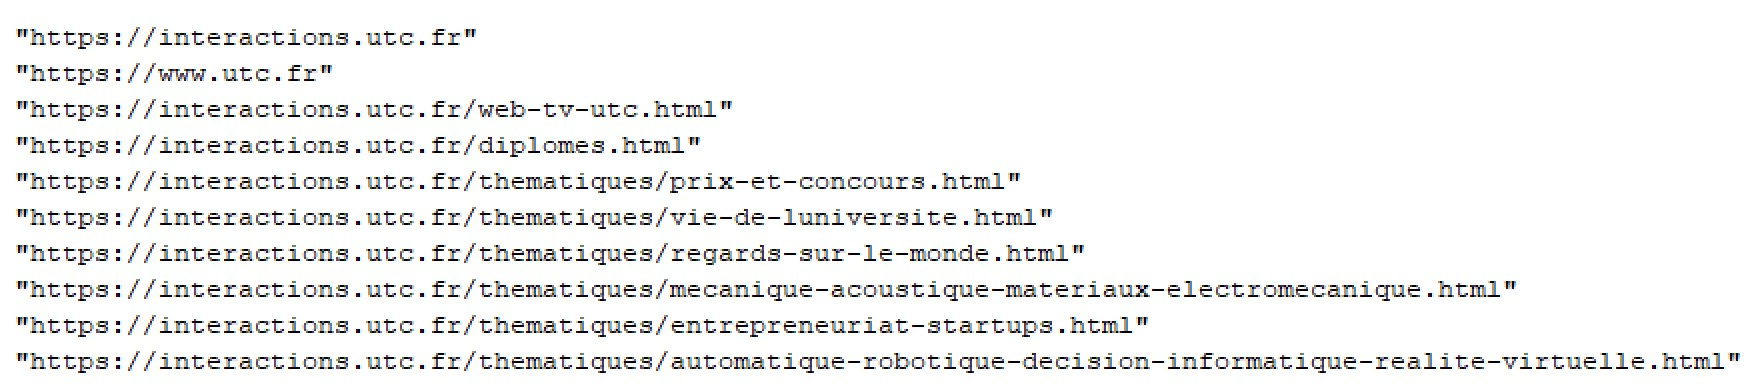
\includegraphics[width=1.1\textwidth]{images/classement.jpg}
              \caption{Classement des 10 pages web de www.utc.fr avec le meilleur score de PageRank}
              \label{fig:gr2}
            \end{figure}
            De plus, on peut tracer également pi afin d'observer les potentiels pics de pages avec un score élevée.
            \begin{figure}[H]
              \centering
                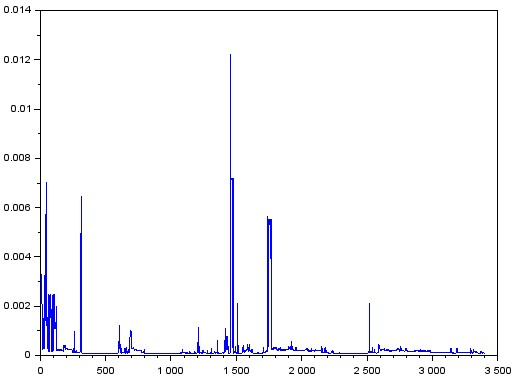
\includegraphics[width=0.6\textwidth]{images/pi.jpg}
              \caption{Classement des 10 pages web de www.utc.fr avec le meilleur score de PageRank}
              \label{fig:gr3}
            \end{figure}
            Finalement, cet algorithme, couplé à une fonction de recherche de caractères dans les URL, permet d'avoir une première approche d'un moteur de recherche plus ou moins fonctionnel. En utilisant la fonction search.sce fournit en TD, on peut, par exemple, avoir un premier aperçu du classement des pages comportant le mot "mathematiques" dans leur URL :
            \begin{figure}[H]
              \centering
                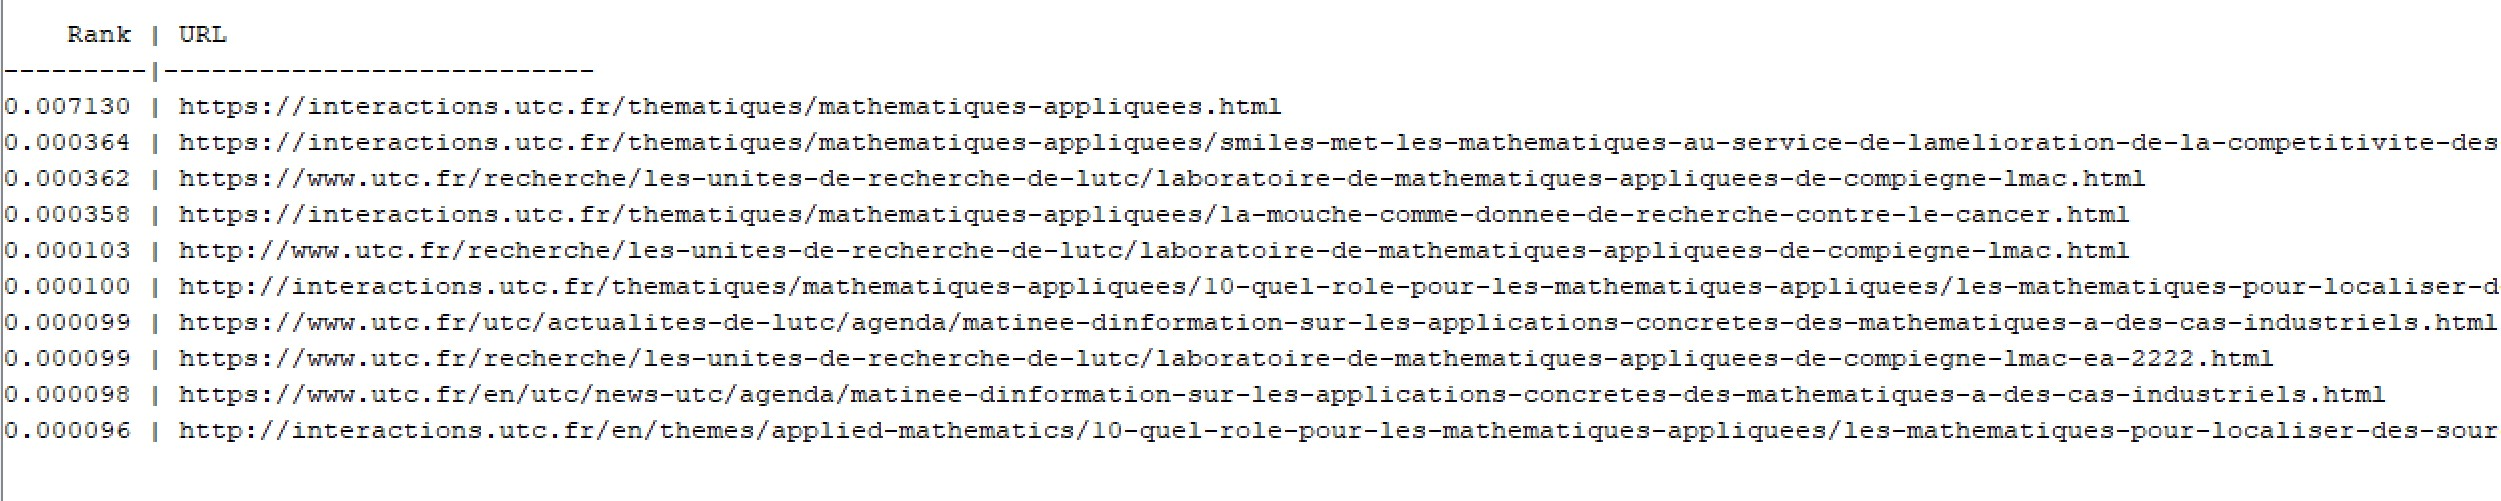
\includegraphics[width=1\textwidth]{images/classement2.jpg}
              \caption{Classement des pages web de www.utc.fr comportant le mot clé "mathematiques" dans leur URL}
              \label{fig:gr4}
            \end{figure}
   \newpage
   \section*{Conclusion}
   \phantomsection
   \markboth{Conclusion}{}
   \addcontentsline{toc}{section}{Conclusion}
      Finalement, l'UV MT94 a été une agréable surprise pour ma part, elle est pour moi l'aboutissement des notions mathématiques étudiées au cours du tronc commun à l'UTC et permet de mieux visualiser et ainsi, comprendre des concepts purement théoriques.\\\\Souhaitant, par la suite, étudier dans la branche informatique de l'UTC et plus particulièrement dans le domaine de l'IA, cette UV et ce projet m'ont permis de me renseigner, et d'ores et déjà, comprendre certains algorithmes et techniques pour le machine learning. \\\\Je regrette de ne pas avoir pu traiter et approfondir toutes les notions vu en cours et en TD, faute de temps, mais j'ai pu toutefois en avoir une introduction qui me permettra d'avoir des fondamentaux dans mes enseignements futurs.\\\\
      Pour conclure, j'aimerais remercier encore une fois M.Stéphane Mottelet pour m'avoir permis de suivre cette UV le semestre précédant mon entrée en branche.
   
   \newpage
    \section*{Références}
    \phantomsection
    \addcontentsline{toc}{section}{Références}
    \markboth{Références}{}
    \begin{itemize}
        \item Cours de MT94, Stéphane Mottelet
        \item \href{https://mpsib-camille-guerin.pagesperso-orange.fr/Python/Mandelbrot/Mandelbrot.pdf}{"Mandelbrot", 2019}
        \item \href{https://www2.mat.ulaval.ca/fileadmin/Cours/MAT-2430/Notes_de_cours/NotesDeCours.pdf}{"Introduction aux fractals
et aux systèmes dynamiques", Jean-Jacques Gervais, 2009}
        \item \href{https://fr.wikipedia.org/wiki/Ensemble_de_Mandelbrot}{"Ensemble de Mandelbrot", Wikipedia}
        \item \href{https://sebastianraschka.com/pdf/lecture-notes/stat453ss21/L05_gradient-descent_slides.pdf}{"Fitting Neurons with
Gradient Descent", Sebastian Raschka, 2021}
        \item \href{https://brilliant.org/wiki/backpropagation/}{"Backpropagation", Brillant}
        \item \href{https://hagan.okstate.edu/NNDesign.pdf}{"Neural Network Design 2nd Edition", Martin T. Hagan, Howard B. Demuth, Mark Hudson Beale, Orlando De Jesús, 2014}
    \end{itemize}








